\documentclass[11pt,a4paper]{article}

%% ── Packages ─────────────────────────────────────────────────
\usepackage[margin=2.5cm]{geometry}
\usepackage{amsmath,amssymb,amsthm,mathtools}
\usepackage{bm}
\usepackage[T1]{fontenc}
\usepackage{lmodern,microtype}
\usepackage[colorlinks=true,
            linkcolor=blue!60!black,
            citecolor=blue!60!black,
            urlcolor=blue!60!black]{hyperref}
\usepackage[numbers]{natbib}
\usepackage{booktabs,array,multirow,rotating}
\usepackage{enumitem}
\usepackage{xcolor}
\usepackage{tcolorbox}
\usepackage{algorithm,algpseudocode}
\usepackage{pdflscape}
\usepackage{graphicx}
\usepackage{float} % explicit dependency for the [H] placement specifier used throughout

%% ── Theorem environments ─────────────────────────────────────
\newtheorem{definition}{Definition}[section]
\newtheorem{theorem}[definition]{Theorem}
\newtheorem{proposition}[definition]{Proposition}
\newtheorem{remark}[definition]{Remark}
\newtheorem{implementation}[definition]{Implementation}

%% ── Macros ───────────────────────────────────────────────────
\newcommand{\R}{\mathbb{R}}
\newcommand{\N}{\mathbb{N}}
\newcommand{\E}{\mathbb{E}}
\newcommand{\Q}{\mathbb{Q}}
\newcommand{\T}{\mathbb{T}}
\renewcommand{\O}{\mathbb{O}}
\newcommand{\PP}{\mathbb{P}}
\newcommand{\F}{\mathcal{F}}
\newcommand{\cL}{\mathcal{L}}
\newcommand{\DLV}{\boldsymbol{\Sigma}}
\newcommand{\logDLV}{\boldsymbol{\Lambda}}
\newcommand{\thetat}{\boldsymbol{\theta}}
\newcommand{\zt}{\mathbf{z}}
\newcommand{\Xt}{\mathbf{X}}
\newcommand{\BS}{\mathrm{BS}}
\newcommand{\softplus}{\mathrm{softplus}}
\newcommand{\logsig}{\mathrm{LogSig}}
\newcommand{\BSCall}{\mathrm{BSCall}}
\newcommand{\diag}{\mathrm{diag}}
\renewcommand{\P}{\mathbb{P}}
\renewcommand{\Q}{\mathbb{Q}}
\DeclareRobustCommand{\supstack}[2]{\stackrel{\mbox{{\scriptsize ${#1}$}}}{ {#2} }}     % symbol over another
\DeclareRobustCommand{\eqlabel}[1]{\label{eq:#1}}                                     % an equation label
\DeclareRobustCommand{\eq}[1]{\begin{equation}\eqlabel{#1}}                           % start an equation
\DeclareRobustCommand{\eqx}{\begin{equation}}                                         % start an equation no label
\DeclareRobustCommand{\eqend}{\end{equation}}                                         % end an equation


%% ── Title ────────────────────────────────────────────────────
\title{%
  \textbf{DYSANOS}\\[6pt]
  \large 
Generative Dynamic Smooth Arbitrage-free Non-parametric Option Surfaces
}
\author{%
  Hans Buehler\thanks{%
    Mathematical Institute and Oxford-Man Institute,
    University of Oxford.
    \texttt{hans.buehler@maths.ox.ac.uk}}
  \and
  Blanka Horvath\thanks{%
    Mathematical Institute and Oxford-Man Institute,
    University of Oxford. \texttt{blanka.horvath@maths.ox.ac.uk}}
  \and
  Anastasis Kratsios\thanks{%
    McMaster University and Vector Institute.}
    \and
  Magnus Wiese\thanks{%
    Mathematical Institute,
    University of Oxford. \texttt{magnus.wiese@maths.ox.ac.uk}}
}
\date{\today\\Version 2.0}

%% ============================================================
\begin{document}
\maketitle

%% ── Abstract ────────────────────────────────────────────────

\begin{abstract}
This article presents with DYSANOS the first generative market model 
for smooth SANOS option surfaces for all strikes and expiries which are
free of static arbitrage. 
Our model is designed to generate entire paths of daily spot and option prices for years
in the future. 

We present a robust and useful if somewhat simplistic baseline in the form of an AR(1) model.
We discuss model setup, data pipeline, and training and investigate market
reconstruction, stability, and tail behavior. We illustrate model performance
on 891 Option Metrics IvyDB S\&P Index surfaces from 2022 to~2025, drawn from
an underlying archive beginning in 2020.
With explicit 1D--4D expiry nodes, the two-$\eta$ affine-200 model places
80.9\% of 3.57 million quotes inside bid--ask.
Finally, a no-replay scalar log-variance diffusion recovers much more of the
observed tail mass and tail persistence than Gaussian innovations, although it
still underproduces two- and three-week extremes.  Block-randomization tests of
decoded 2025 surface paths do not reject Gaussian, heavy-tail, diffusion, or
historical-replay candidates at the 5\% level.
For a reduced, 45-instrument tradable universe we further construct, via
Deep Hedging, a near-martingale measure whose empirically re-solved objective
value is statistically indistinguishable from zero, a first, deliberately
scoped step towards a risk-neutral DYSANOS.
\end{abstract}

\tableofcontents
\bigskip\hrule\bigskip

%% ============================================================

% \newpage 
\section{Introduction}
\label{sec:intro}
%% ============================================================

The implied volatility surface of an option market changes dynamically over time, giving rise to
Vega risk when risk managing option portfolios.
Modelling the dynamics of a full continuous surface of options
in a way that is simultaneously \emph{statistically realistic} and \emph{statically
arbitrage-free} at every simulated date has remained an open problem since the
foundational work of~\cite{ContVol} on dynamics of the implied volatility surface.

\begin{figure}[H]
    \centering
    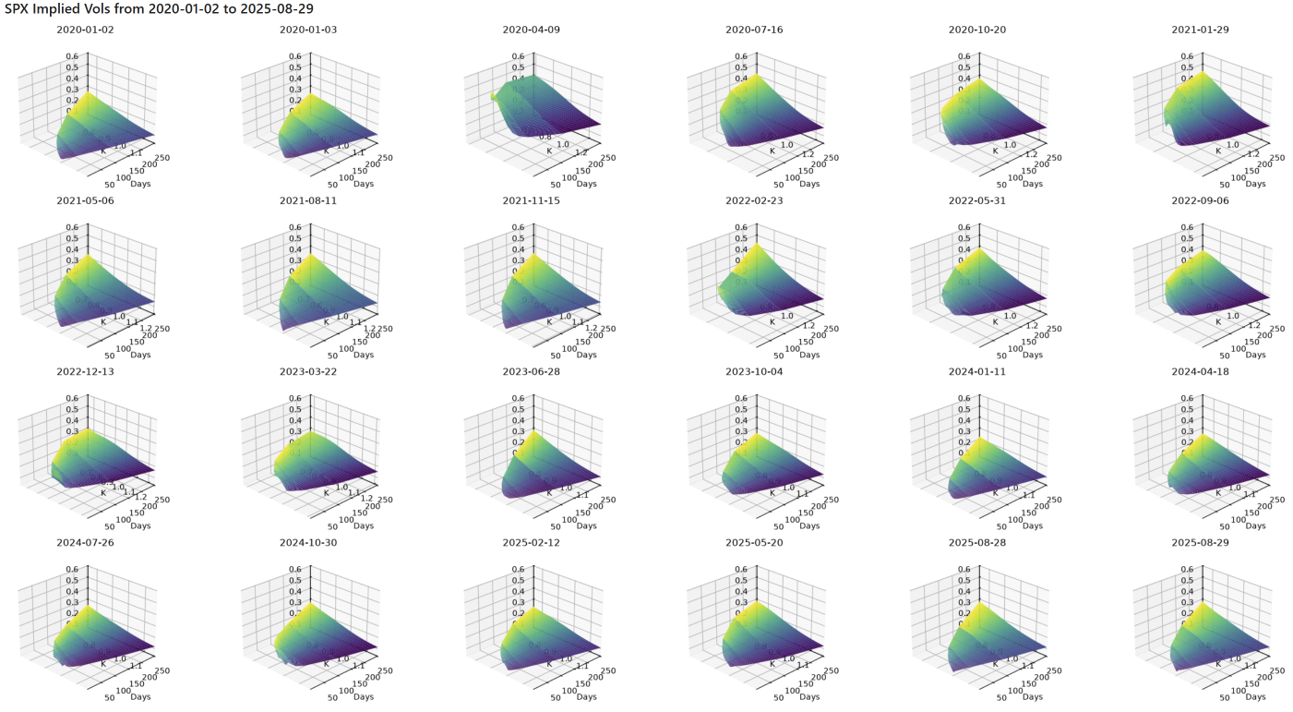
\includegraphics[width=0.9\linewidth]{SPX2020-2025.png}
    \caption{Historical implied volatilities for mid-prices of S\&P~500 Index options
    from 2020-01-02 to 2025-08-29
    using Option Metrics Ivy DB data via WRDS \url{https://wrds-www.wharton.upenn.edu/} (the latest data available at the time of writing).}
    \label{fig:initialexample}
\end{figure}

The most advanced approach until recently were the simulators~\cite{wiese2019simulate,wiese2021multiassetspotoptionmarket,Cohen02012023} 
for realistic dynamics of
a \emph{discrete floating grid} of options which are strictly
 arbitrage-free at each simulation date. These simulators are using, in essence, the discrete local volatility
representation pioneered in~\cite{DLV} to ensure absence of static arbitrage in every simulated
option surface. 


However, the restriction of the above models to a discrete set of floating option strikes and time-to-expiries
means that the simulators do not have access to the daily returns $dC_t(\tau,k)$
of an actual tradable instruments with cash strikes $k$ and calendar expiries~$\tau$ (because the
contract terms change from one simulated day to another).  It therefore does
not directly provide statistically consistent time series of fixed-contract
returns, which are required to validate simulated dynamics against observed
market returns.
Of course, since the discrete option prices are free of arbitrage, one option would be 
to interpolate option prices linearly, which means all options are free of static arbitrage.
However, as shown in~\cite{buehler2006expensive} and illustrated in~\cite{SANOS2026}
linear interpolation yields the most expensive possible arbitrage-free price for any
option off the grid, rendering the approach unsuitable in practice. Being linear
also means that the implied probability density is piecewise constant and zero between strikes.
In other words
the spot price can only take values at the model strikes for each expiry to avoid dynamic
arbitrage.

This article presents a model framework for
\begin{itemize}
    \item  \textbf{(i) realistic generative dynamics} of
    \item  \textbf{(ii) smooth option surfaces for all strikes and expiries} which are
    \item  \textbf{(iii) free of static arbitrage}.
\end{itemize}
%
We also comment on finding a risk-neutral measure for a subset of traded options.
This article is a refinement of material presented at The XIII Bachelier World Congress in Bologna.\footnote{\url{https://quantitative-research.de/dl/DYSANOS.pdf}}

\subsection*{Historic Context and Literature Review}

\paragraph{The classical approach and its limitations.}
Quantitative finance has traditionally approached this problem by specifying
analytically tractable risk-neutral dynamics for the underlying asset ---
Heston, rough volatility, SABR --- and then \emph{calibrating} model parameters
to fit each day's option surface independently. They are then overlaid with 
a local volatility surface using the seminal~\cite{Guyon2011TheSC}. The latter
guarantees that all options are initially priced correctly.

In this paradigm, realistic surface dynamics are an afterthought: calibration is repeated
from scratch on each date. 
This approach is both impractical for large-scale simulation and structurally inconsistent
with the goal of generating realistic implied volatility or option price
paths.

\paragraph{Simulating Implied Volatility.}
A natural data-driven alternative is to treat the implied volatility surface itself
as the simulation object, much as implied in~\cite{ContVol}.
The fundamental difficulty is that there is no known parametrization  of
the implied volatility surface which is strictly free of static
arbitrage. There exists numerous attempts to rectify this with classic (e.g.~\cite{fengler2009}) and machine learned
methods (e.g.~\cite{vae_ning2023arbitrage}) but to our knowledge none of them can strictly guarantee absence of static arbitrage.

If a simulated surface admits a butterfly spread or calendar spread arbitrage,
then a learning agent can exploit an artificial profit which is unrelated to the
problem for which the generated market was intended. Aside from those classic constraints
call prices also need to adhere to boundary conditions which are often not discussed
in the literature (we repeat them below).

Most published works also simplify the problem by only considering few strikes and expiries.

\paragraph{Constrained Parameter Spaces and Code Books.}
The core challenge of any representation of an option prices surface is that no-static-arbitrage conditions are essentially
linear conditions on call prices, which are difficult to enforce directly in a generative machine learning model. 
This challenge is shared by most representations including most parametrizations of implied volatility.

The idea of a ``code book'' as introduced in~\cite{TangentLevy} is to find a representation of the option price surface
which is numerically tractable for simulation and for which required parameter constraints are straight forward to enforce.
Indeed, the seminal~\cite{TangentLevy} achieves that goal. In addition, the authors are able to also
construct a risk-neutral measure consistent with the code book representation.
They achieve this, essentially, by writing the spot price as a product of independent increments. That construction unfortunately also restricts
the dynamics their model can represent. It tends to fit poorly to statistical data due to the strong cross-expiry correlation of implied forward volatilities.

\paragraph{Local Volatility as a Code Book.}
An intuitive alternative is to use Dupire's local volatility as ``code book'' instead 
\emph{(not as dynamical model)}. Given a non-negative local volatility function
$\sigma_t(T,K)$ for $(T,K)\in\R^2_{\geq 0}$ defined on some day~$t$
we can define 
a smooth, strictly arbitrage-free option surface 
$C_t(T,K):=C^\mathrm{LV}(\sigma_t;T,K)$ 
by solving the Dupire forward-PDE
$\partial_T C^\mathrm{LV}(\sigma_t;T,K)
 = \mbox{$\frac12$}K^2\sigma_t^2(T,K)\,
   \partial^2_{KK}C^\mathrm{LV}(\sigma_t;T,K)$.
That means any statistical generative model of Dupire's local volatility gives rise
to a dynamic model of option surfaces which are by construction free of static arbitrage.

However, in order to price any simulated option off a simulated local volatility surface
we would need to solve a forward-PDE on a suitably
fine grid which is slow, particularly when used within batch-based gradient descent training.

The idea to address this conundrum is to use a grid of options and define a discrete version
of local volatility on that grid, which is what we called
\emph{discrete local volatility (DLV)} in~\cite{DLV}. 
It is essentially the discretized local volatility which is consistent with using an implicit forward-PDE operator on a sparse inhomogeneous grid of options,
as explained in~\cite{AndreasenHuge}.
However,
its native option prices for strikes not on its base grid are the result of linear interpolation and therefore, as mentioned above, ``too expensive''.
We therefore use
our smooth SANOS extension~\cite{SANOS2026}.

The use of SANOS also allows to fit our model very efficiently to observed bid/ask spreads over the entire observed option surface.

\subsection*{Key contributions}


\subsubsection*{SANOS Decoder:}
    We show how to implement and learn a coordinate transformation of
    our SANOS~\cite{SANOS2026} model 
    such that the ``ML-SANOS'' state parameters $h_t$ live in an unconstrained space 
    $\R^{d}$.  The call
    prices 
    $$
        h_t \longmapsto C(h_t;T,K)  \ .
    $$    
    remain smooth and statically arbitrage-free.
    
    We show how ML-SANOS can be trained directly to suitably pre-processed 
    option market data, yielding a trained $h_t$ for each day.
    The pre-processing step means that DYSANOS, via SANOS, is fitted to real market bid/ask prices.
    
\subsubsection*{Generative Dynamics}
    We fit a stable weekly AR(1) directly to the learned
    surface state. Its transition is parameterized as the matrix exponential
    of a dissipative generator, and its full innovation covariance is learned
    by a nonsingular Cholesky factor. The resulting stationary law permits
    exact Gaussian transitions at daily, weekly, or longer horizons; as
    non-Gaussian alternatives, a no-replay log-variance diffusion is fitted
    and historical one-week innovations can be resampled.
    
    We do not
    claim that this approach provides the most realistic dynamics; rather,
    we see this implementation as baseline to beat with more modern
    time series models.

\subsubsection*{Risk-Neutral Dynamics}

Every decoded SANOS surface is free of static arbitrage by construction.
We show that we can ``remove the drift'' in the sense of~\cite{removedrift} for a subset of the (infinite) tradable instruments
by finding a near-martingale measure~$\Q$ equivalent to the learned~$\P$ such that a
Deep Hedging~\cite{DH} agent cannot make any money trading under~$\Q$.


%% ============================================================
\section{DYSANOS}
%% ============================================================

\label{sec:markets}


We consider European call options on a single underlying
for historic days $t\in \{t_1,\ldots,t_m\}$.
We assume forwards, discount factors, and survival probabilities
are deterministic. As described in remark~\ref{rem:driftless}.
 we can therefore convert them at each point~$t$ to driftless equivalents
where spot, forwards, discount factors and survival probabilities are all one, for every~$t$.


At time~$t$, we observe~$L_t\in\N$ 
European call option prices with time-to-expiries $T_t^\ell \geq 0$ and
relative strikes $K_t^\ell\geq 0$
for $\ell=1,\ldots,L_t$
in the market. Their symbolic payoff is therefore
$$
   \left(\frac{S_{t+T_t^\ell}}{S_t} - K_t^\ell \right)^+ \ .
$$
We denote by $B_t^{\ell}$ and $A_t^\ell$ their bid and ask prices;
mid-price and half-spread are defined (in vector notation) as
$C_t := \tfrac{1}{2}(A_t + B_t)$ and
$\gamma_t := \tfrac{1}{2}(A_t - B_t)$.

We generally assume that $B_t\succ0$ and $\gamma_t\succ0$.\footnote{
We define $x \succ y \Leftrightarrow \forall i: x^i > y^i$.}
Contrary to most derivative literature, we do not assume that bid/ask prices are in some way free of arbitrage; instead
we will show how to handle arbitrage valuations gracefully.

We will use the Black~\&~Scholes formula in terms of \emph{total volatilities} defined 
for a spot $S$, strike~$K$ and total volatility~$W$ as
\begin{equation}\label{eq:bs}
    \BSCall(S,K,W) := S\,\mathcal{N}( d_+ ) - K\,\mathcal{N}(d_-)
    \ \ \ \mbox{for} \ \ \
    d_\pm := \frac{ 1 }{ W } \log K/S \pm \frac12 W^2 
\end{equation}
where~$\mathcal{N}$ denotes the normal distribution function.

\begin{remark}[Conversion to driftless data]\label{rem:driftless}
  Assume that at each time $t$ spot is $S_t$, forwards are $F_t(T)$, discount factors are $B_t(T)$,
  and survival probabilities are $Q_t(T)$. It was shown in~\cite{BuehlerVolAndDivs} that if cash dividends 
  are present then, conditional on no default, spot at $T$ splits as $S_T = \big(F_t(T)-D_t(T)\big) X_T + D_t(T)$
  for a non-negative martingale $X$ with $X_t=1$, where $D_t(T)$ represents the discounted floor value of all
  cash dividends paid between $t$ and $T$.

  We note that even in the presence of default risk put-call parity holds. Hence for any put $\tilde P_t(T,\tilde K)$ with time-to-expiry $T$ and cash strike $\tilde{K}$ 
  let $\tilde C_t(T,\tilde{K}) = \tilde P_t(T,\tilde{K}) + B_t(T)\, Q_t(T)\, F_t(T) - B_t(T)\, \tilde{K}$.

  Assume then that $\tilde C_t(T,\tilde{K})$ denotes the market call price for time-to-expiry~$T$ and cash strike~$\tilde K$. 
  Define the ``pure'' strike normalized to a unit forward and discount factor as
  $$
  K := \frac{ \tilde K - D_t(T) }{ F_t(T) - D_t(T) }  \ .
  $$
  Accordingly, the ``pure'' call price is given as
  $$
    C_t(T,K) := \frac{\tilde{C}_t\Big(T,\, K\big(F_t(T)-D_t(T)\big) + D_t(T)\Big)}{B_t(T) \, Q_t(T)\,\big(F_t(T)-D_t(T)\big)} \ .
  $$
 See~\cite{BuehlerVolAndDivs} for details and proof.
\end{remark}

\subsection{Arbitrage-Free Call Price Functions}

A~call price function is simply a function $C:\R^2_{\geq} \longrightarrow  \R_{\geq 0}$
which computes call prices $C(T,K)$ for time-to-expiries $T\geq 0$ and relative
strikes $K\geq 0$ (i.e.~the call prices are normalized to a spot price of~$1$). 
The objective of this section and the next is to generate such functions $C_t$ for each
simulated date~$t$ such that each $C_t$ is ``free of static arbitrage'' in the following sense:

\begin{definition}
A call price surface $C: \R^2_{\geq 0}\to \R_{\geq 0}$ is \emph{free of static arbitrage} if there is no trade
which has non-negative returns with a non-zero probability of
positive returns.    

This is equivalent to the existence of a
martingale~$Z$ such that $C(T,K)= \E\big[(Z_{T}-K)^+\big]$.
\end{definition}

\begin{theorem}\label{th:arbfree}
A call price surface $C$ is free of static arbitrage if and only if 
it does not admit negative butterfly or calendar
spreads and satisfies the boundary conditions
$C(T,0)=1$, $C(0,K)=(1-K)^+$, $\lim_{K\uparrow\infty} C(T,K)=0$ and $\partial_K C(T,0)\in[-1,0)$.

The stricter condition~$\partial_K C(T,0)=-1$ applies if the stock price cannot become zero.
\end{theorem}

This has been proven in~\cite{buehler2006expensive}. Remark~\ref{rem:actionable_arbitrage} 
shows that these conditions each are not superfluous: we give a practical
guide on how to construct \emph{actionable} arbitrage strategies if any of the above
are violated. 

\begin{remark}[Actionable arbitrage if the conditions of theorem~\ref{th:arbfree} are not met]\label{rem:actionable_arbitrage}
All of the below are meant as practical heuristics.
\begin{itemize}
    \item \textbf{Butterfly arbitrage:} this means that the price of a positive
    butterfly payoff is negative. The arbitrage is to get paid to enter into 
    the butterfly which can only ever generate a positive return.

    \item \textbf{Calendar arbitrage:} if for the same strike $K$ 
    the call price at $T_2$ is below the call price
    at $T_1$, then:
    \begin{enumerate}
        \item 
            Sell the call at $T_1$ and buy the call at $T_2$. This provides
            a positive cash flow $\pi_0>0$.
        \item 
            In $T_1$ if the call expiries out of the money, then we have made money: both
            $\pi_0$ and a potential positive payoff at $T_2$ in our favour.

            If the call expires in the money, then we deliver one share
            and receive $K$. We are now short that share.
            In $T_2$, if the call expiries in the money, then we receive one share
            to cover our short in return for $K$. Our total cashflow is $\pi_0$.
            If the call expiries out of the money, then $S_T<K$. We can therefore
            buy back the share and cover our short for less than $K$.
            Our profits are $\pi_0+(K-S_T)^+>0$.
    \end{enumerate}
    \item If $C(0,K) \not= (1-K)^+$ we have an immediate pathological arbitrage.
    \item If $C(T,0)>1$ then sell the call and cover with one share; if $C(T,0)<1$
    then buy the call and enter into a short equity position.

    \item $\partial_K C(T,0)\geq -1$: assume on the contrary there is a $K\downarrow 0$
    such that $(1-C(T,K))/(-K) < -1$ i.e.~$C(T,K) = 1-K - \epsilon$ for some $\epsilon>0$.
          Buy the call and short sell the equity, resulting a cash position of $\pi_0=-K+\epsilon$;
          the payoff in $T$ is $(S_T-K)^+$ which allows us to cover our position and cash
          with a total reward of~$\epsilon>0$.

    \item $\partial_K C(T,0)<0$: assume on the contrary there is a $K\downarrow 0$
    such that $(1-C(T,K))/(-K) \geq 0$. We show existence of
    arbitrage in the case of equality
    i.e.~existence of some~$K>0$ such that $C(T,K)=1$.
    In that case we sell the call and buy the equity for~$1$.
    If the call expires in the money, we deliver the share
    and receive $K>0$. If the call expiries out of the money, then sell
    the share for $S_T\geq 0$.

    \item $\lim_{K\uparrow \infty} C(T,K) = 0$ which means for all $c>0$
    there exists some $K$ such that $C(T,K')<c$ for all $K'\geq K$ (because of convexity).
    This is the only arbitrage condition which is technical because a violation means, 
    essentially, that the equity can grow without bounds which violates
    integrability.
    Assume therefore on the contrary 
    that there is some~$c>0$ such that $C(T,K)\geq c$ for all $K$. 
    Notice that, formally,
    $$
        S_T = - \int_0^\infty \frac{ (S_T-K+dK)^+ - (S_T-K)^+ }{ dK } dK
            = S_T + \lim_{K\uparrow \infty} (S_T-K)^+ \ .
    $$
    Therefore sell (a discretization of) the strip
    $$
    \int_0^\infty \frac{ C(T,K) -  C(T,K+dK) }{ dK } dK = 1 + e
    $$
    which delivers~$S_T$, and buy the equity. This will generate profits of~$e>0$.
 \end{itemize}
\end{remark}

\subsection{SANOS - Smooth Arbitrage-free Non-parametric Option Surfaces}
\label{sec:sanos}

In~\cite{SANOS2026} we introduced a  non-parametric family
of call price functions which are all statically arbitrage-free. For clarity, let us briefly fix $t$ and drop it from the notation of market data
and model parameters.

Each call price function is given in terms of model expiries
$0 = \hat T^0 < \hat T^1 < \cdots < \hat T^M$ and, for each model expiry,
$N^j>0$ inner strikes.\footnote{Note that we changed notation slightly vs.~\cite{SANOS2026}.}  Including the two boundary strikes, write
$\hat K^j = (\hat K^{j,i})_{i=0,\ldots,N^j+1}$. It is recommended that the two outer strikes
are far away from the inner strikes.\footnote{
    In our experiments, the inner strikes
    $0<\hat K^{j,1}<\cdots<1<\cdots<\hat K^{j,N^j}$
    were chosen first and then extended by $\hat K^{j,0}:=\hat K^{j,1}/2$ and
    $\hat K^{j,N^j+1} = 1.5\,\hat K^{j,N^j}$.
}  Model strikes and expiries do not need to match
market strikes or expiries. See~\cite{SANOS2026} for general comments on grid construction.

We say that $q=(q^1,\ldots,q^M)$ with $q^j\in\R^{N^j+2}$ is a \emph{martingale density} if
it satisfies the linear constraints
\begin{equation}\label{eq:qocnd}
    \left\{
    \begin{array}{ll}
        \mbox{Each $q^j$ is a density:} & q^j\geq 0,\ (q^j)'1 = 1 \\
        \mbox{Each $q^j$ has unit expectation:} & (q^j)' \hat K^j=1 \\
        \mbox{The $q$ are in convex order:}&
            {q^j}' CX_j \geq {q^{j-1}}' CX_{j|j-1}
            \\
    \end{array}
    \right.
\end{equation}
The matrices $CX_j$ and $CX_{j|j-1}$ project the density on call prices. They are defined as
$$
CX_j^{i,k} := (\hat K^{j,i}-\hat K^{j,k})^+ \ \ \ i=0,\ldots,N^j+1;\ k=1,\ldots,N^j 
$$
and
$$
CX_{j|j-1}^{i,k} := (\hat K^{j-1,i}-\hat K^{j,k})^+ \ \ \ i=0,\ldots,N^{j-1}+1;\ k=1,\ldots,N^j  \ . 
$$
Accordingly, ${q^j}' CX_j \in \R^{N_j}$ is the vector of call prices for strikes $\hat K^{j}\in\R^{N_j}$ computed using the density $q^j$
while ${q^{j-1}}' CX_{j|j-1} \in \R^{N_j}$ is the vector of call prices for the same strikes $\hat K^{j}\in\R^{N_j}$ computed using the previous density $q^{j-1}$.
The condition ${q^j}' CX_j \geq {q^{j-1}}' CX_{j|j-1}$ enforces that call prices are increasing into each strike $\hat K^{j}$.

\begin{definition}[SANOS call price]
\label{def:sanos}
Let $q$ be a martingale density and $0<W^1< \cdots < W^M$
be increasing smoothing total volatilities.\footnote{The linear-programming preprocessing uses 50\% of ATM total volatility. The trained ML-SANOS decoder instead learns the positive forward smoothing multipliers $\eta^j$.}
The SANOS call price 
 for arbitrary $T\geq0 ,K\geq 0$ 
is given by
\begin{equation}
  \label{eq:sanos_interp}
  \begin{aligned}
  C(T,K):={}&\alpha^j(T)\sum_{i=0}^{N^j+1}
       \BSCall\!\bigl(\hat K^{j,i},K,W(T)\bigr)q^{j,i}\\
     &+(1-\alpha^j(T))\sum_{i=0}^{N^{j-1}+1}
       \BSCall\!\bigl(\hat K^{j-1,i},K,W(T)\bigr)q^{j-1,i},
       \qquad T \in (\hat T^{j-1},\hat T^j].
  \end{aligned}
\end{equation}
with $\alpha^j(T) = (T - \hat T^{j-1})/(\hat T^j - \hat T^{j-1})$
and total volatility $W(T) := \alpha^j(T) W^j + (1-\alpha^j(T)) W^{j-1}$.

For $T>\hat T^M$ we
set $\alpha^{M+1}(T)=0$ and $W(T):=W^M\sqrt{T / \hat T^M}$; however extrapolation beyond
the last model expiry is generally not recommended.

For $T<\hat T^1$ we
set $\alpha^1(T)=0$ and $W(T):=W^1\sqrt{T / \hat T^1}$; however extrapolation before
the first model expiry is generally not recommended.

\end{definition}


\begin{theorem}
    The call price function $C$ is statically arbitrage-free.
For $W(T)>0$ it is $C^\infty$ in $K$. The function is as smooth as~$\alpha$ in~$T$.
\end{theorem}

\begin{remark}
    Contrary to~\cite{SANOS2026} we interpolated the Black \& Scholes backbone in total volatility linearly, not variance.
    This is a mechanical choice to avoid taking square roots of variables during training
    which can lead to exploding gradients. If forward volatilities are bounded well away from
    zero, linear interpolation in variance is suitable, too.
\end{remark}

\begin{remark}
    The Black~\&~Scholes formula in~\eqref{eq:sanos_interp} can be replaced
    by the call price function for any martingale in~$T$, for example the FFT Heston price formula~\cite{carrmadan1999}.
    For practical implementations, the
    function should be fast on a GPU.
\end{remark}

\paragraph{Calibration as a linear program:}
 We assume we obtain $W^1<\cdots<W^M$
from the market e.g.~as square roots of ATM variance per expiry.
Given~$W$ the model call price $C^\ell := C(T^\ell, K^\ell)$ for a market expiry $T^\ell$ and
a market strike $K^\ell$
can be seen in~\eqref{eq:sanos_interp}
to be linear in~$q$.
The market-fitting problem can therefore be formulated as the linear programme
\begin{equation}
  \label{eq:lp}
  \min_{q} \sum_\ell \frac{
    (C^\ell - \bm{A}^\ell)^+ + (\bm{B}^\ell - C^\ell)^+ + \epsilon |C^\ell - \bm{M}^\ell|
  }{ (A^\ell - B^\ell)/2}
\end{equation}
subject to the linear constraints~\eqref{eq:qocnd} encoding non-negativity, normalisation, integration to~$1$, and the inter-expiry convex-order constraints that enforce absence of calendar-spread
arbitrage. We note that the model strikes and time-to-expires do not need to correspond
to market strikes or expiries.\\

As discusssed in~\cite{SANOS2026} the primary application of this model is \emph{interpolation}: if the model strikes
are are superset of \emph{all} strikes of relevant market instruments then the model can practically be fit to the
vast majorty of options accross the entire surface from 1 day to expiries to several years. Stronger, if the model is
linear ($W=0$) the existence of the densities $q$ is equivalent to absence of arbitrage with respect to the market bid/asks (usually
this simply means our market data is not aligned correctly).

On S\&P~500 Index data with 1000 options across 48 expiries (2-day to 657 business-day TTE),
the LP solves in sub-seconds on a desktop PC, achieving 91.4\% of options within
bid--ask on a representative date (2025-05-06), with a median error of 21\% of the
half-spread on the remaining options. Figure~\ref{fig:sanos_fit} illustrates
the quality of the fit. The example is from~\cite{SANOS2026}; refer to that work for further details.
\begin{figure}[H]
    \centering
    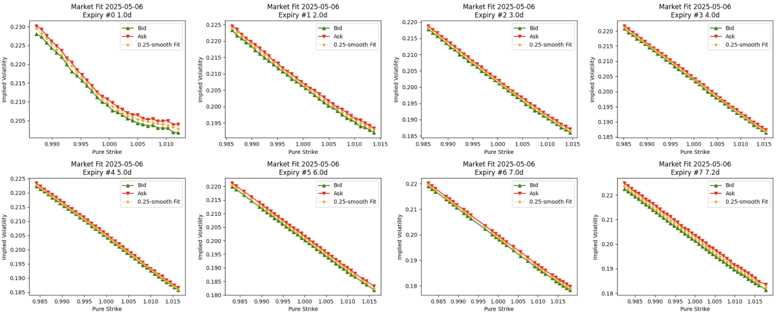
\includegraphics[width=0.9\linewidth]{fit-short.png}\\
    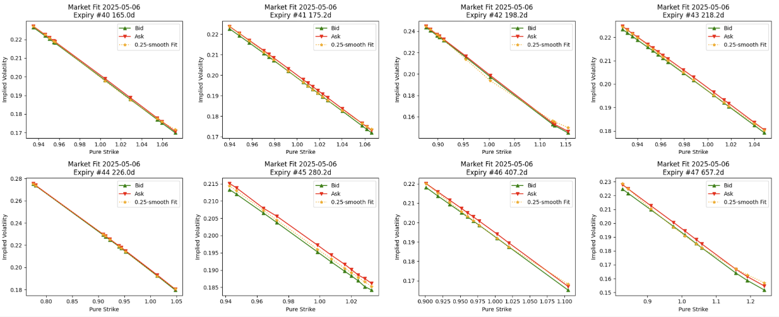
\includegraphics[width=0.9\linewidth]{fit-long.png}
    \caption{Example fit of SANOS.}
    \label{fig:sanos_fit}
\end{figure}

\section{ML-SANOS}
\label{sec:mlsanos}

We may view our  SANOS call price operator as a map from the model
parameters to a function space
\begin{equation}\label{eq:sanosmap}
    \big( q, W;\, \hat K,\hat T\big) \supstack{\mathrm{SANOS}}\longmapsto C    
\end{equation}
for which we naturally want to learn $q,W$ and, as we will see, $\hat K$ (as the right strike grid
depends on the implied variance of the market).
However, the density weights $q^j$ in particular are subject to the linear constraints~\eqref{eq:qocnd}
for which no exact methods exist to integrate them into standard batch gradient descent methods.
In this section we therefore reparameterize the map~\eqref{eq:sanosmap} in terms
of learnable parameters.

To do so, we no longer require strict \emph{interpolation} of the market prices. While we will want to be as close as possible
to observed market prices (and will show that we are able to do so), we now focus on a model parametrization which lends itself
to efficient learning using standard optimization techniques. That means that the number of strikes must somehow be kept manageable,
rather than be dictated by the number of market instruments at each observed historic day~$t$.

As a first step we therefore fix a common strike grid $\hat K$ with $0<\hat K^0<\cdots<1<\cdots<\hat K^{N+1}$ across expiries to simplify our model.
The call price for strike $\hat K^i$ given the density $q^j$ is given as $c^{j,i} = (q^j)'(\hat K - \hat K^i)^+$.
The convex order condition in~\eqref{eq:qocnd} therefore becomes simply $c^{j,i} \geq c^{j-1,i}$ for all $i$.

We now reparameterize our densities in terms of \emph{discrete local volatilities (DLVs)}~\cite{DLV}: let
$$     
    \omega^{i\pm} := \pm    \frac{ (\hat K^{i})^2 }{ (\hat K^{i+1} - \hat K^{i-1})\,(\hat K^{i\pm 1} - \hat K^{i}) }  \geq 0
$$
and with it the tridiagonal matrix~$\Omega$ with 
\begin{itemize}
    \item Upper diagonal $( -\omega^{1-}, \ldots, -\omega^{N-}, 0 )$,
    \item Lower diagonal $( 0, -\omega^{1+}, \ldots, -\omega^{N^j+} )$, and
    \item Main diagonal $( 0, +\omega^{1+}+\omega^{1-}, \ldots, 1+\omega^{N^j+}+\omega^{N^j-}, 0 )$.
\end{itemize}
i.e.
\eqx
    \Omega = \left(
                \begin{array}{cccccccccc}
                0 & -\omega^{1-} & 0 \\
                0 & +\omega^{1+}+\omega^{1-} & -\omega^{2-} \\
                0 & -\omega^{1+} & +\omega^{2+}+\omega^{2-} \\
                & & & &  \ddots\\
                & & & &  \ddots\\
                & & & & & +\omega^{(N-1)+}+\omega^{(N-1)-} & -\omega^{N-} & 0 \\
                & & & & & -\omega^{(N-1)+} & +\omega^{N+}+\omega^{N-} & 0 \\
                & & & & & 0 & -\omega^{N+} & 
                \end{array} 
    \right) \ .
\eqend
Then for \emph{any} squared (discrete) local volatilities $\Sigma^j = ( 0, \Sigma^{j,1}, \ldots, \Sigma^{j,N}, 0 )$
the operator
\eqx
            1 + \Omega\ \mathrm{diag}(\Sigma^j) (\hat T_j - \hat T_{j-1}) \in \R^{(N+2)\times(N+2)}
\eqend
is a tridiagonal operator with positive main diagonal and negative off diagonals. 
It is basically the discrete implicit scheme for the forward equation of the continuous time Dupire SDE.
It is well known~\cite{DLV}
that this operator is invertible, and the inverse~$\Xi^j$ can be efficiently computed on GPU using a compiled
Thomas' algorithm. It is also
a martingale transition operator in
 the sense of~\cite{DLV} which means that the densities $q^1,\ldots,q^M$ generated 
 iteratively starting in $q^0=(1)$ by
\begin{equation}\label{eq:densitytrans}
    q^j = \Big( 1 + \Omega\ \mathrm{diag}(\Sigma^j) (\hat T_j - \hat T_{j-1}) \Big)^{-1} q^{j-1} 
\end{equation}
form a martingale density over~$\hat K$.

With the above we have established a map from much simpler non-negative discrete local vols squared to
densities, and then to SANOS call prices:
\begin{equation}\label{eq:sanosmap2}
    \big( \Sigma, W;\, \hat K,\hat T\big) \supstack{\mathrm{DLV}}\longmapsto
    \big( q, W;\, \hat K,\hat T\big) \supstack{\mathrm{SANOS}}\longmapsto C \ .
\end{equation}
That allows us to pass to a practically unconstrained parameter set, which we call the ML-SANOS parametrization.
We will use the sigmoid function $\mathrm{sigmoid}(x)=(1+e^{-x})^{-1}$.

\begin{definition}[ML-SANOS]\label{def:ml-sanos}
    Fix the normalized grid geometry for ML-SANOS with:
    \begin{itemize}
        \item Time-to-expiries (TTEs) $0=\hat T^0<\cdots<\hat T^M$ with
        $\Delta\hat T^j = \hat T^j-\hat T^{j-1}$;
        \item Normalized strikes $z^1<\cdots<0<\cdots<z^N$ which we assume contain zero;
        \item Minimum and maximum forward volatilities $\sigma_{\max} > \sigma_{\min} > 0$; 
        \item Minimum and maximum squared discrete local volatilities $\Sigma_{\max} > \Sigma_{\min} > 0$; and
        \item Minimum and maximum smoothing factors $1> \eta_{\max} > \eta_{\min} \geq 0$.
    \end{itemize}
    We translate the new real-valued ML-SANOS parameters
    $u=(u^\Sigma,u^\sigma,u^{\eta,\mathrm f},u^{\eta,\mathrm{term}})
    \in\R^{M\times N}\times\R^M\times\R^2$ into SANOS parameters as follows:
    \begin{itemize}
        \item Total volatilities: 
        define the \textbf{forward volatilities}
             \eqx
                    \sigma^j := \sigma_{\min}
               +\mathrm{sigmoid}( u^{\sigma,j} ) ( \sigma_{\max} - \sigma_{\min} )
            \eqend
            and two smoothing factors
            \begin{equation}
                \label{eq:etatrans}
                \eta^{\mathrm f}:=\eta_{\min}
                  +(\eta_{\max}-\eta_{\min})
                    \mathrm{sigmoid}(u^{\eta,\mathrm f}) \ \ \ \mbox{and} \ \ \
                \eta^{\mathrm{term}}:=\eta_{\min}
                  +(\eta_{\max}-\eta_{\min})
                    \mathrm{sigmoid}(u^{\eta,\mathrm{term}}) \ .
            \end{equation}
            With these quantities define the \textbf{total volatilities}
             \begin{equation}\label{eq:totalW}
             \widetilde W^j := \sum_{\ell=1}^{j} \sigma^\ell \sqrt{\Delta\hat T^\ell}
             \qquad\mbox{and}\qquad
             W^j := \eta^{\mathrm f} \sigma^1 \sqrt{\Delta\hat T^1}\ + \eta^{\mathrm{term}} \sum_{\ell=2}^{j}  \sigma^\ell \sqrt{\Delta\hat T^\ell}\ .
             \end{equation}
        \item We use $\widetilde W^j$ to define a fixed grid as \textbf{relative strikes}
              \begin{equation}\label{eq:constructK}
                \hat K := \exp\left( z \widetilde W^1 \right) \bigcup \exp\left( z^i \widetilde W^M \right) \ ,
              \end{equation}
              sufficiently sorted, 
              with boundaries $\hat K^{0}:=\frac12 \hat K^{1}$ and $\hat K^{N+1} := \frac32 \hat K^{N}$.
        \item Finally, we use the new real-valued ML-SANOS parameters to define the \textbf{squared discrete local volatilities}:
              \begin{equation}\label{eq:defDLVdsq}
                 \Sigma^{j,i}
                 :=\min\!\left\{\Sigma_{\max},
                    \Sigma_{\min}+\exp(u^{\Sigma,j,i})\right\}\ .
              \end{equation}
              (This formulation avoid saturation of the sigmoid function as the raw log-DLV coordinate approaches the cap  $\Sigma_{\max}$;
              it requires adding a penalty term to the loss function.)

    \end{itemize}
    Put together, this process describes a map
    \begin{equation}
        \big(\,u;z,\hat T\,\big)  \supstack{
            \begin{array}{c}
                \mathrm{ML}\\
                \mathrm{SANOS}
                \end{array}
        }\longmapsto \big(\, \Sigma,W;\,\hat K,\hat T \big) 
        \supstack{\mathrm{DLV}}\longmapsto \big(\,q,W;\,\hat K,\hat T \big)  \supstack{\mathrm{SANOS}}\longmapsto C \ .
    \end{equation}
    In our new parametrization $u$ lives in an unrestricted space and is therefore
    particularly suited for ML/AI based learning.  The expiry locations remain fixed.
\end{definition}

In our
experiments we use the bounds
$(\Sigma_{\min},\Sigma_{\max})=(0.01^2,3^2)$,
$(\sigma_{\min},\sigma_{\max})=(0.01,1)$, and
$(\eta_{\min},\eta_{\max})=(0.01,0.50)$. 

\subsection{Learning ML-SANOS from real data}
\label{sec:learning-ml-sanos}

Our new parameterization allows the model to fit not only DLV's but also forward volatilities and, via~$u^\eta$ the size of the strike grid
for a given set of market data. This extension means the model is no longer linear in its parameters. We therefore fit it with 
stochastic gradient descent methods.

\paragraph{Model specifications}

We apply this to two model specifications: one with weekly expiries only and one with weekly expiries and daily expiries in the front week. The purpose
of this comparison is to assess whether a purely weekly model can capture front dynamics natively. The specific model expiries are:
\begin{align*}
  \text{weekly:}\quad
    &(5,10,15,\ldots,70)\text{i.e.~ $M=14$ business days},\\
  \text{daily+weekly:}\quad
    &(1,2,3,4,5,10,15,\ldots,70)\text{ i.e.~ $M=18$ business days}.
\end{align*}
We use $N=200$ strikes computed using~\eqref{eq:constructK} for $z$ strikes within $(-3,2)$.
The native coordinates are:
\begin{equation}
  u_t=\left(
u_t^{\Sigma},\,
            u_t^{\sigma},\,
      u_t^{\eta}
      \right)
  \in\R^{M(N+1)+2}.
  \label{eq:production-native-state}
\end{equation}
The weekly model therefore has 
2,816 native coordinates while the the daily+weekly model has 3,620 native
coordinates.  
For each geometry we learn a ``direct'' representation $u_t$ for each historic date. We also learn
an additional ``affine-200''
fit with representation
\begin{equation}
  u_t=b+B h_t,
  \qquad h_t\in\R^{200},
  \label{eq:affine-decoder}
\end{equation}
in terms of learned $h_t\in\R^{200}$,
and shared $b\in\R^{M(N+1)+2}$ and
$B\in\R^{(M(N+1)+2)\times200}$.\footnote{
The choice of 200 is an empirical capacity compromise rather than a structural
claim about the intrinsic dimension of option surfaces.  It is large enough
to preserve almost all of the direct native quote fit while remaining below
the number of historical dates, so a full innovation covariance and stable
joint state dynamics can still be estimated.  We report the native-versus-200
fit loss explicitly below rather than treating this dimension as exact.
}


\paragraph{Data and model geometries}

The empirical population sourced from WRDS' Option Metrics Ivy data base contains 891 S\&P~Index dates from 2022-01-03 through
2025-08-29. See appendix~\ref{app:data-pipeline} for our baseline pipeline we use for all our research with this data set.

In addition to the general filters, we here also exclude options ourside the model's strike range (which is effectively $(-3,2)$ NMS) and any options expiring
past the last model expiry of~70 business days. We also exclude tomorrow's AM-settled options. 

We retain 3,566,258 original call-or-put book observations for the daily+weekly model and 3,566,742 for the weekly model.\footnote{
  The slight difference in retained observations arises from the difference in the effective strike range for each model.
}
All options are represented in call-equivalent units through put–call parity; call and put books at the
same expiry and strike remain separate observations and contribute separate loss terms.

\paragraph{Objective Function}

For quote $\ell$ on date $t$, let $ C_t^\ell$ be the decoded option
price, $M_t^\ell=( A_t^\ell+ B_t^\ell)/2$, and
$\gamma_t^\ell=( A_t^\ell- B_t^\ell)/2$. We fit in principle the same
objective as in~\eqref{eq:lp}:
\begin{equation}
  \mathcal L_t^{\mathrm{quote}}
  =
  \frac{1}{L_t}\sum_{\ell=1}^{L_t}
  \frac{(C_t^\ell- A_t^\ell)^+
    +( B_t^\ell-C_t^\ell)^+
    +0.05|C_t^\ell-M_t^\ell|   
  }{ ( A_t^\ell- B_t^\ell)/2 }  
  \label{eq:production-quote-loss} 
\end{equation}
The native controls first fit an independent $u_t$ on every date.  The
affine-200 model jointly updates
$b$, $B$, the historical states $h_t$, and the stable weekly dynamics in
Section~\ref{sec:dynamics}.  A gauge penalty controls the affine
non-identifiability by keeping the fitted states at zero mean and unit
population covariance across the historical dates.

\begin{remark}[Full Objective]
  Two regularization penalties were used.  First, write
  \begin{equation}
    u_{\max}^{\Sigma}:=\log(\Sigma_{\max}-\Sigma_{\min}),
    \qquad a:=0.10,
    \qquad s:=0.35,
  \end{equation}
  and, for every raw log-DLV coordinate, define the smooth one-sided cap
  residual
  \begin{equation}
    r_t^{j,i}
    :=\frac{a}{s}\,
      \log\!\left(
        1+\exp\!\left(\frac{u_t^{\Sigma,j,i}-u_{\max}^{\Sigma}}{a}\right)
      \right).
  \end{equation}
  With $D=891$ historical dates, the full-data DLV-cap penalty corresponding
  to the equal-date minibatch estimator used in training was
  \begin{equation}
    \mathcal L_{\mathrm{cap}}
    :=\frac{1}{D}\sum_{t=1}^{D}
      \frac12\sum_{j=1}^{M}\sum_{i=1}^{N}(r_t^{j,i})^2,
    \qquad
    \lambda_{\mathrm{cap}}=1.
  \end{equation}
  Pricing itself used the mechanical cap in~\eqref{eq:defDLVdsq}; this smooth
  penalty supplies a restoring gradient to the raw coordinate where the
  capped pricing map is flat.  Far above the cap it approaches a quadratic
  penalty with log-scale standard deviation $s=0.35$, while $a=0.10$ controls
  the smooth transition around the cap.

  Second, let $d=200$ be the affine state dimension and define
  \begin{equation}
    \bar h:=\frac{1}{D}\sum_{t=1}^{D}h_t,
    \qquad
    \widehat\Gamma_h
    :=\frac{1}{D}\sum_{t=1}^{D}
      (h_t-\bar h)(h_t-\bar h)^\top.
  \end{equation}
  The gauge penalty was
  \begin{equation}
    \mathcal L_{\mathrm{gauge}}
    :=\frac{1}{d}\lVert\bar h\rVert_2^2
      +\frac{1}{d}\lVert\widehat\Gamma_h-I_d\rVert_F^2,
    \qquad
    \lambda_{\mathrm{gauge}}=0.10,
  \end{equation}
  Thus the complete regularization penalty was
  \begin{equation}
    \mathcal L_{\mathrm{penalty}}
    =\lambda_{\mathrm{cap}}\mathcal L_{\mathrm{cap}}
     +\lambda_{\mathrm{gauge}}\mathcal L_{\mathrm{gauge}}.
  \end{equation}
  Operationally, training was alternating: the quote update included
  $\lambda_{\mathrm{cap}}\mathcal L_{\mathrm{cap}}$, whereas the dynamics
  update included
  $\lambda_{\mathrm{gauge}}\mathcal L_{\mathrm{gauge}}$.
  The covariance uses the population normalization $1/D$, rather than
  $1/(D-1)$.  This gauge removes translations and non-orthogonal changes of
  scale and shear; orthogonal rotations and reflections remain immaterial.
\end{remark}


\subsubsection{Market fit}
\label{sec:fit}

The primary measure of fit is the excess of the model price relative to the bid--ask spread:
for fitted price $C$, bid $B$, and ask $A$, define excess in
half-spread units by
\begin{equation}
  e(C;B,A)
  :=\frac{(C-A)^+ +(B-C)^+}{(A-B)/2}.
  \label{eq:half-spread-excess}
\end{equation}
Thus $e=0$ exactly when the model price lies inside bid--ask. We compute the percentage of options within bid/ask, and
conditionally of being outside, the mean and median violation.

Table~\ref{tab:aggregate-fit} gives the complete quote-population results for
the fitted two-$\eta$ models.

\begin{table}[H]
\centering
\small
\begin{tabular}{lrrrrr}
\toprule
Model & Quotes & Inside bid--ask & Mean excess & Cond. mean & Cond. median\\
\midrule
Weekly native & 3,566,742 & 73.2678\% & 1.1101 & 4.1525 & 1.4261\\
Weekly affine-200 & 3,566,742 & 72.8728\% & 1.1017 & 4.0612 & 1.3925\\
Daily+weekly native & 3,566,258 & 82.2809\% & 0.3120 & 1.7609 & 0.6920\\
Daily+weekly affine-200 & 3,566,258 & \textbf{80.9211\%} & 0.3229 & 1.6924 & 0.6776\\
\bottomrule
\end{tabular}
\caption{Aggregate fit. Excess is defined by \eqref{eq:half-spread-excess}.}
\label{tab:aggregate-fit}
\end{table}

Affine compression costs only 0.39 percentage points for the weekly geometry
and 1.36 percentage points for the daily+weekly geometry.  By contrast, adding
the four short-end nodes improves affine-200 fit by 8.05 percentage points.
Expiry geometry, not latent-state capacity, is therefore the main bottleneck.

The mechanism is visible directly in table~\ref{tab:short-fit}.

\begin{table}[H]
\centering
\begin{tabular}{lrrrrr}
\toprule
Model & 1D & 2D & 3D & 4D & 5D\\
\midrule
Weekly native & 24.07\% & 32.47\% & 42.04\% & 55.66\% & 45.45\%\\
Weekly affine-200 & 24.35\% & 32.65\% & 42.11\% & 55.26\% & 45.26\%\\
Daily+weekly native & 94.56\% & 95.21\% & 95.57\% & 95.77\% & 68.43\%\\
Daily+weekly affine-200 & 88.59\% & 91.98\% & 93.68\% & 94.13\% & 67.58\%\\
\bottomrule
\end{tabular}
\caption{Inside-spread rates at the five shortest nominal expiries.}
\label{tab:short-fit}
\end{table}

The weekly model has no independent 1D--4D state directions and must
extrapolate from 5D.  The daily+weekly model represents front-end dislocations
explicitly.

Figure~\ref{fig:fit-by-expiry} shows that this is a localized geometry effect,
not a general loss of fit.  The explicit daily nodes lift the 1D--4D
inside-spread rate from roughly 24--55\% to 89--94\% in the affine model.  Once
the market expiry is comfortably beyond the first weekly node, the two
geometries converge and both approach near-complete containment at the longer
end.  Within either geometry, the native and affine-200 curves remain close;
compression is therefore secondary to where the decoder places its expiry
nodes.

\begin{figure}[p]
  \centering
  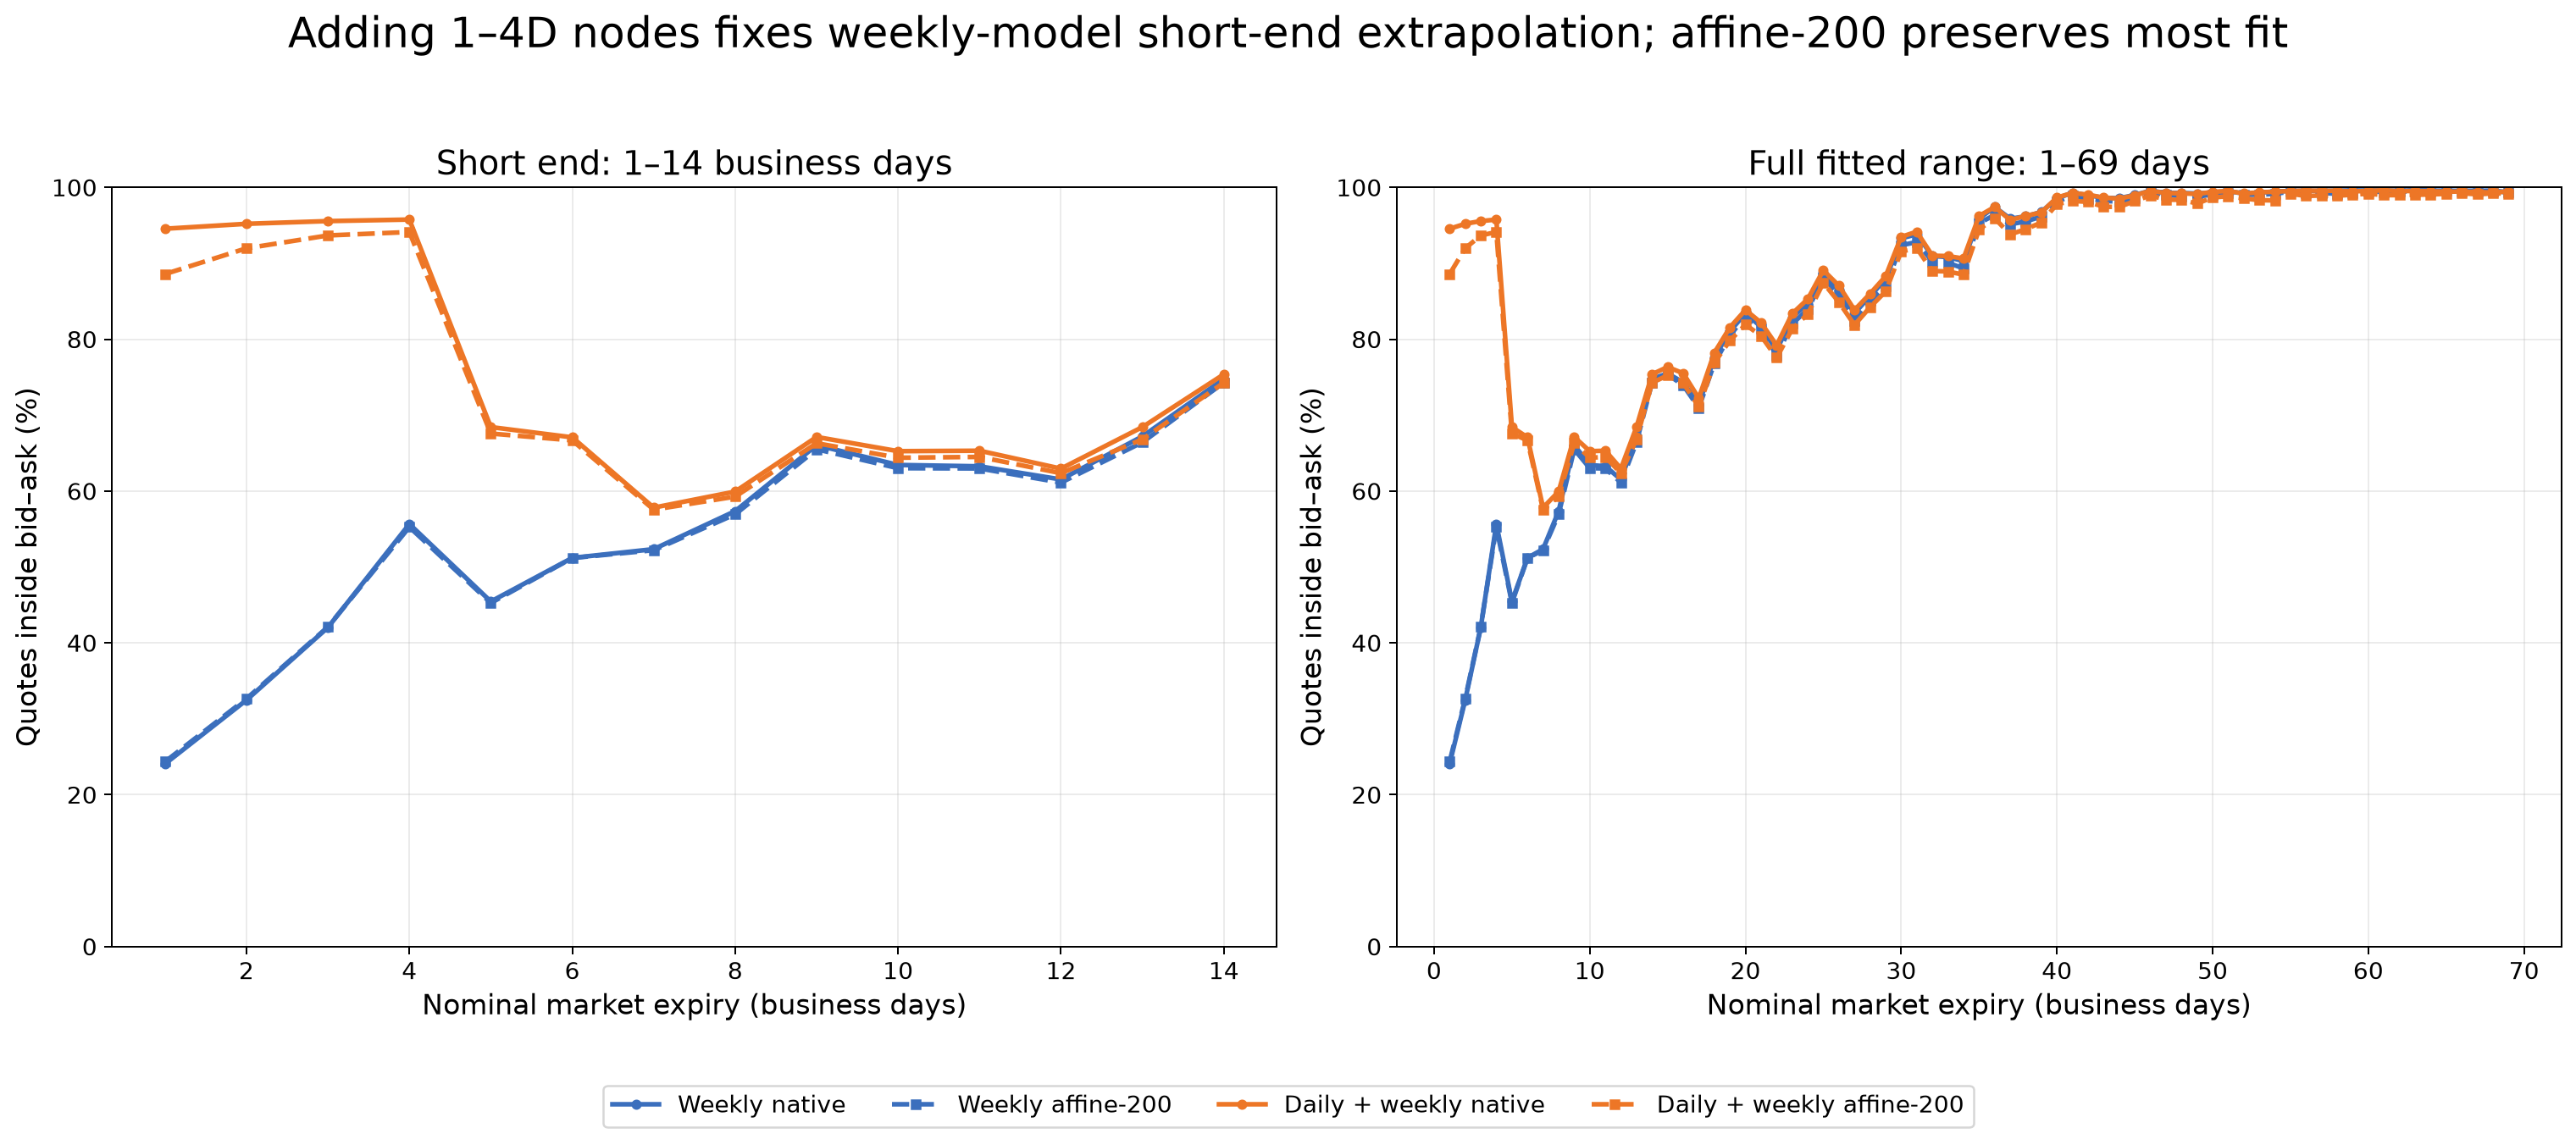
\includegraphics[width=\textwidth]{generated/presentation_market_fit_by_expiry.png}
  \caption{Inside-spread rate by nominal market expiry for the weekly and
  daily+weekly geometries, before and after affine-200 compression.  All
  quote observations in each expiry bucket are included.}
  \label{fig:fit-by-expiry}
\end{figure}

The same conclusion appears in the magnitude of misses.  Conditional on a
quote falling outside the spread, Figure~\ref{fig:excess-by-expiry} measures
its distance in half-spread units.  A weekly decoder forced to extrapolate
before 5D can miss 1D and 2D quotes by more than ten half-spreads on average;
explicit daily nodes reduce that short-end error to roughly one to three
half-spreads.  The gap narrows rapidly after the first week.

\begin{figure}[p]
  \centering
  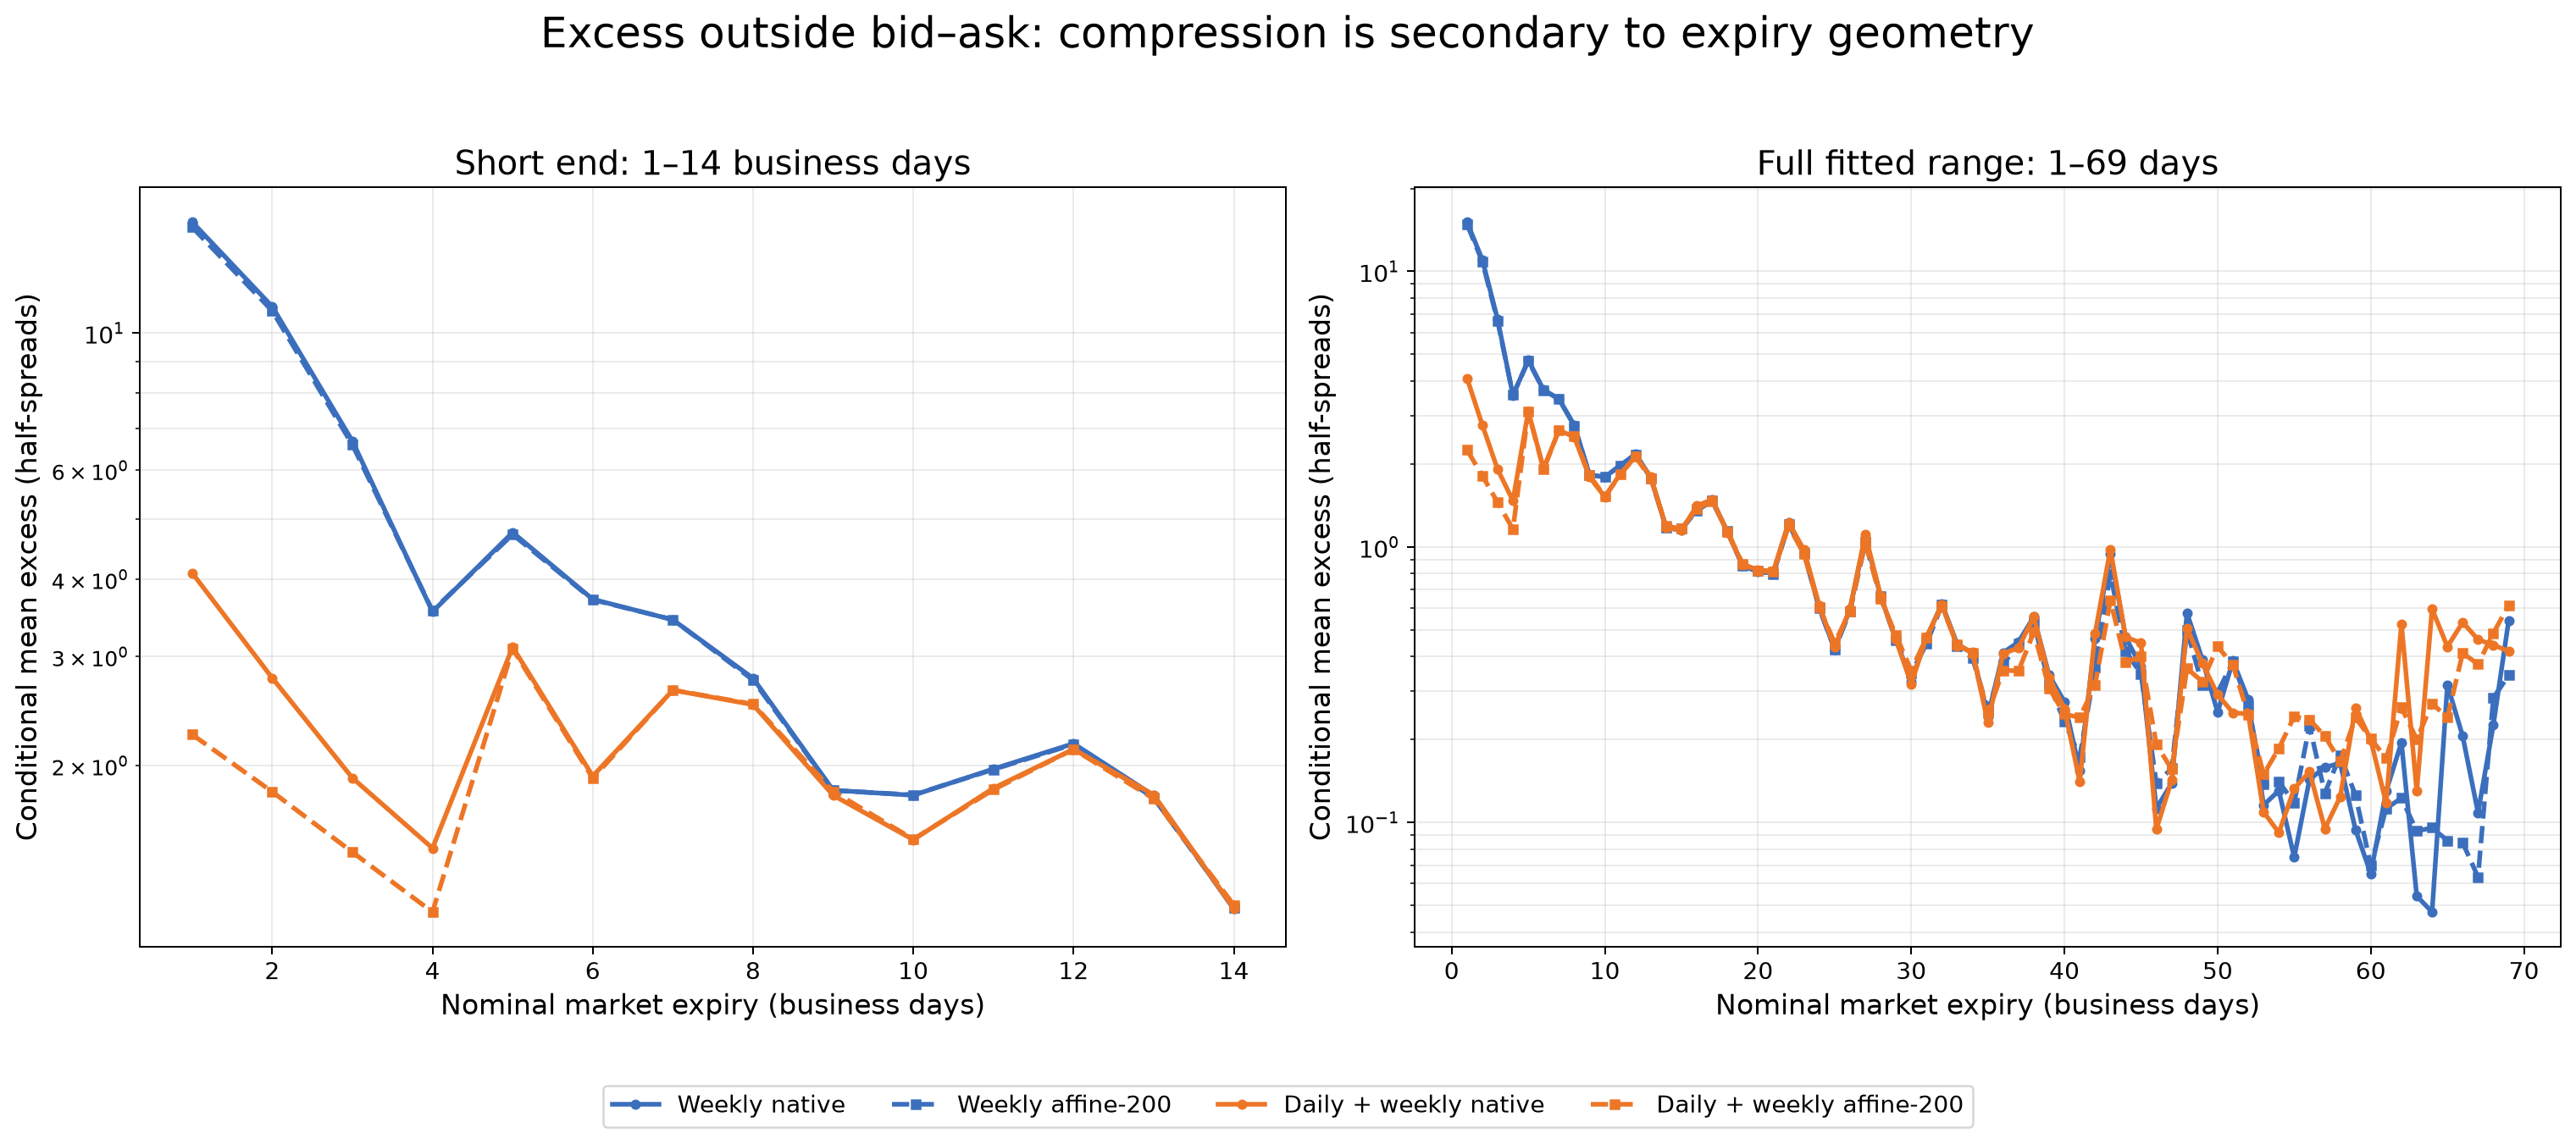
\includegraphics[width=\textwidth]{generated/presentation_excess_by_expiry.png}
  \caption{Mean half-spread excess by market expiry, conditional on the model
  price being outside bid--ask.  The logarithmic vertical scale exposes the
  very large short-end extrapolation errors of the weekly geometry.}
  \label{fig:excess-by-expiry}
\end{figure}

Figure~\ref{fig:representative-fit} gives a cross-sectional view on
2024-06-14.  At representative expiries of 10, 23, 43, and 67 business days,
the independently fitted market SANOS surface and the completed weekly affine
model track one another closely over the central liquid strike range.  The
longer-expiry panels also expose a material discrepancy at the far-left
boundary; the native-versus-affine IV RMSE is 5.30 and 6.87 volatility points
there, compared with 0.12 and 0.30 at 10 and 23 days.  The example therefore
supports the aggregate fit result while making clear that extrapolative wing
coordinates remain a limitation.

\begin{figure}[p]
  \centering
  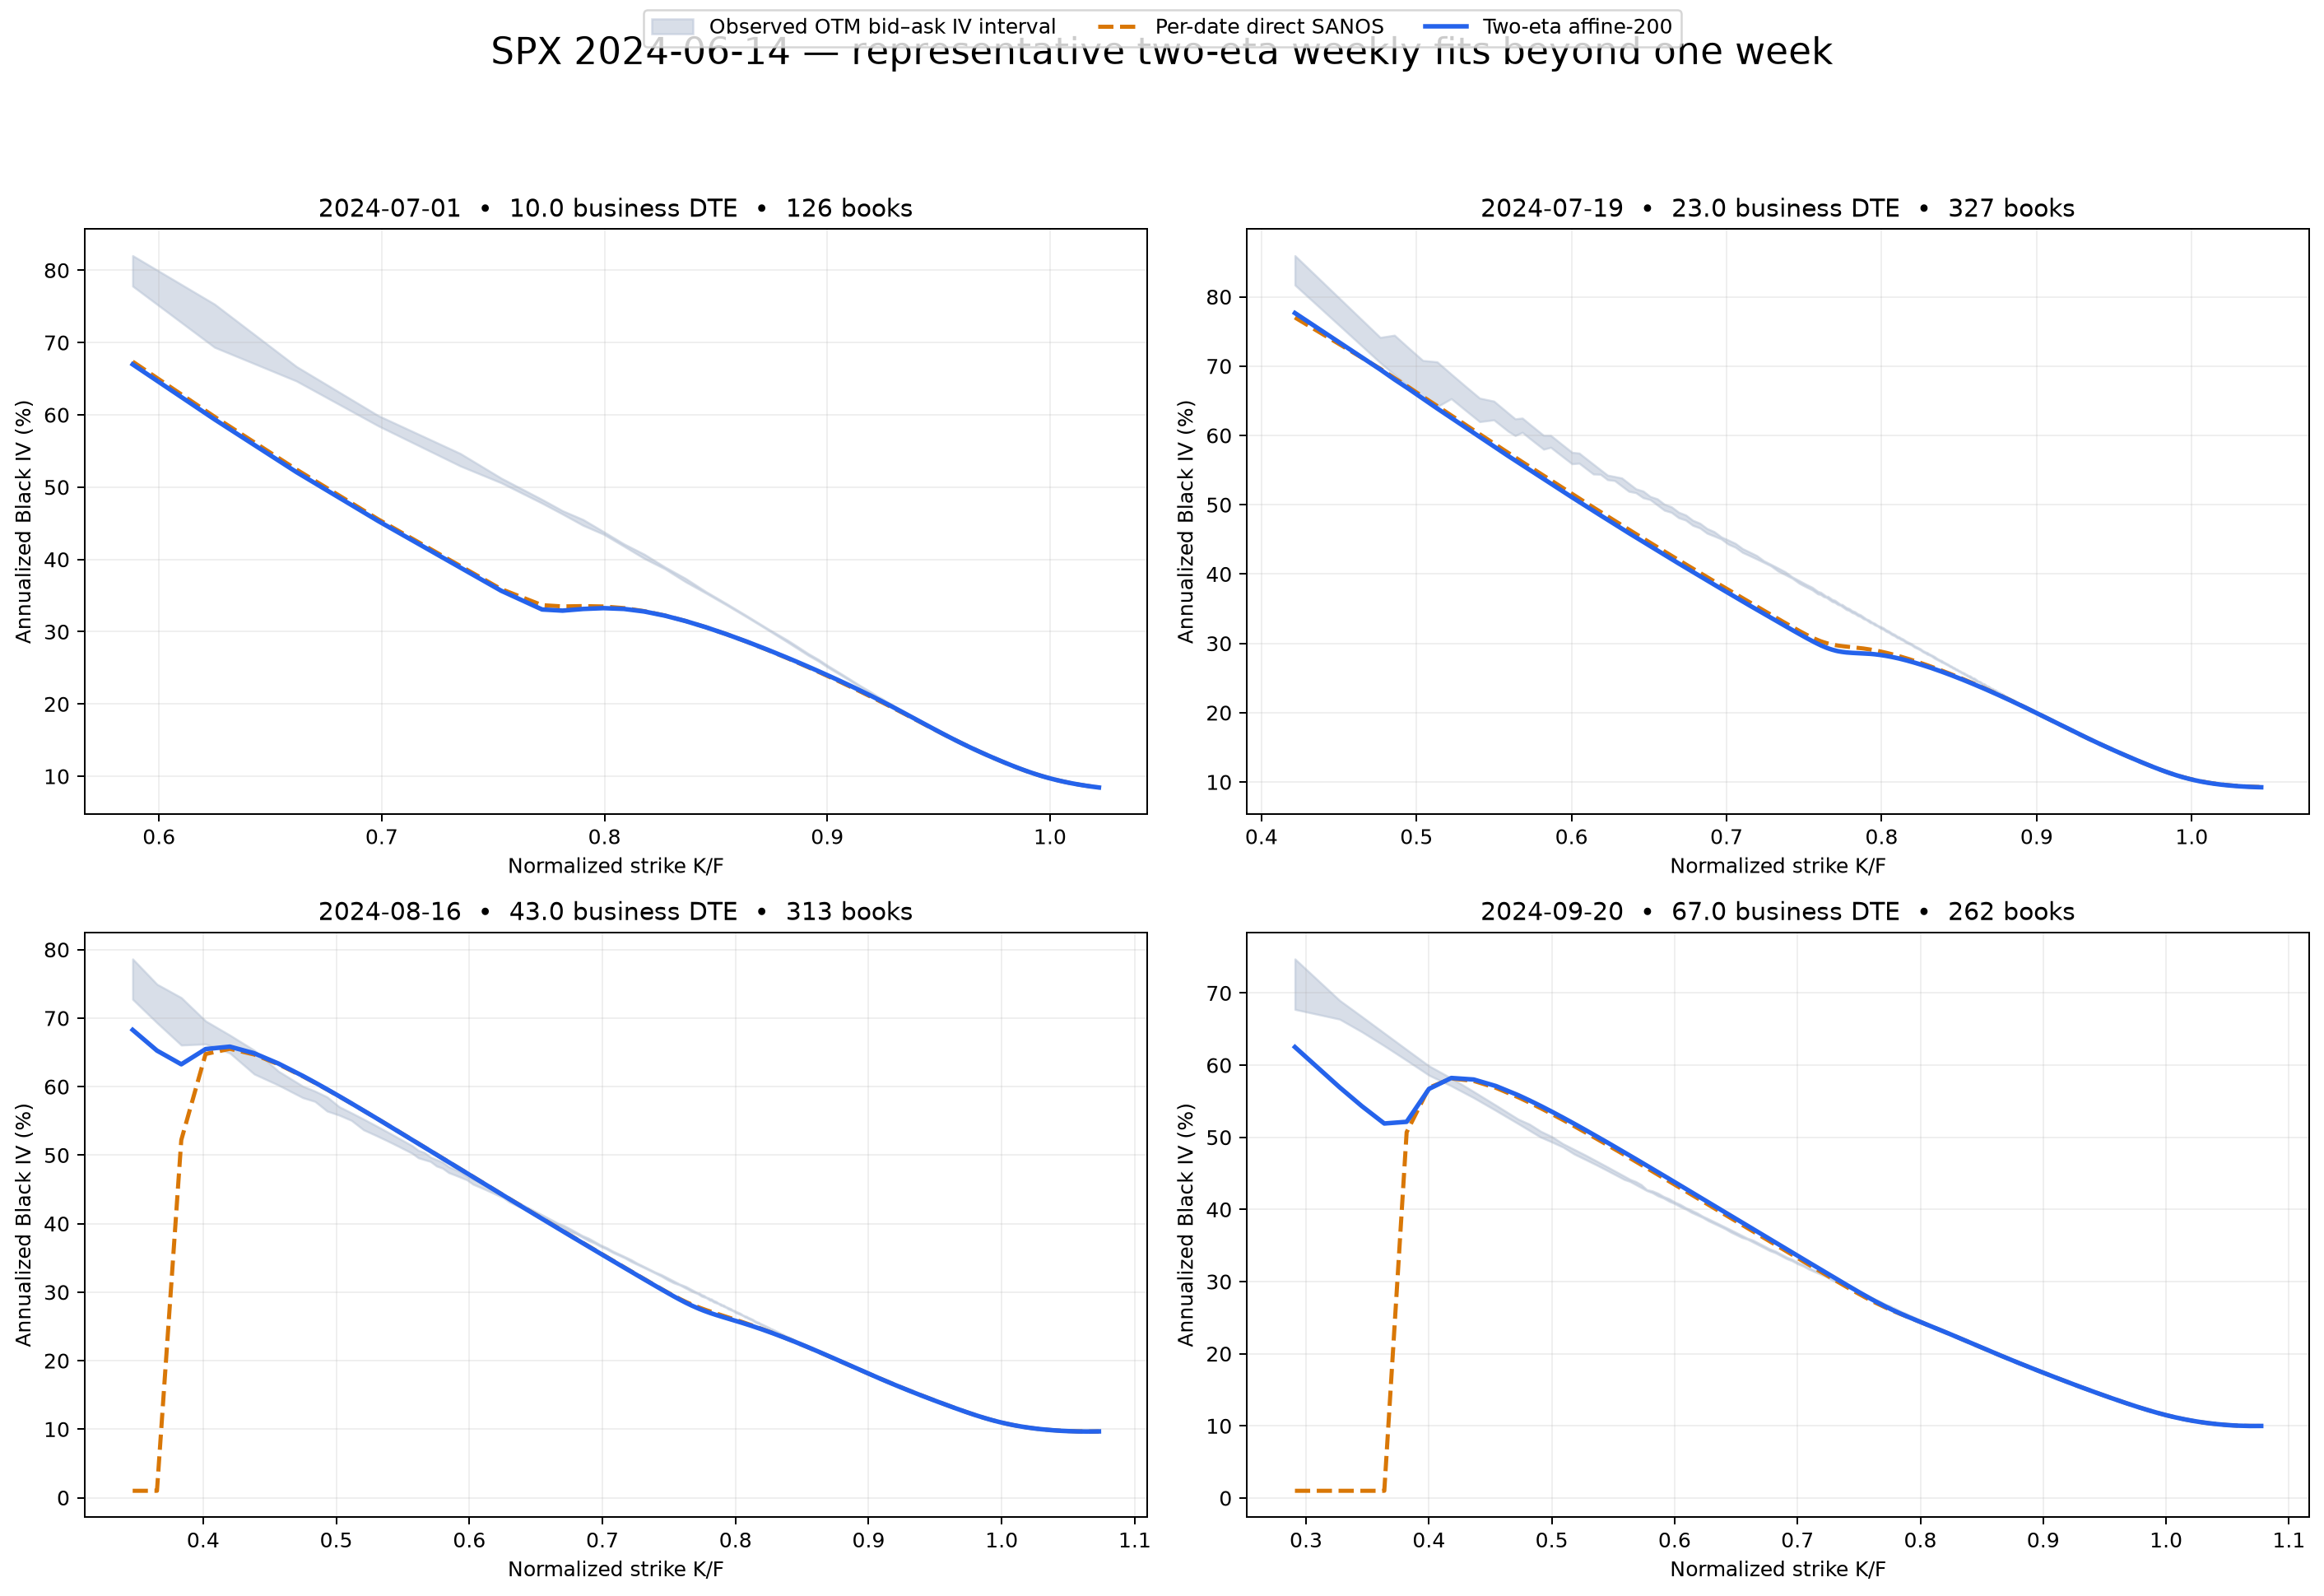
\includegraphics[width=0.92\textwidth]{generated/presentation_representative_surface_fit.png}
  \caption{Representative SPX fit on 2024-06-14.  The panels compare observed
  OTM bid--ask implied-volatility intervals, the per-date SANOS preprocessing
  fit, and the affine weekly model at four market expiries.}
  \label{fig:representative-fit}
\end{figure}

\paragraph{Interpretation of the 80\% number.}
The 80.92\% headline is the affine-compression reconstruction test over the
full 891-date population.  After joint fitting of the stable state dynamics,
the simulation checkpoint places 81.48\% of all quotes inside bid--ask; its
2025 slice contains 707,630 observations and has an 80.56\% inside-spread
rate.  The shared decoder and dynamics used all dates, so the latter is a
chronological slice rather than a strict temporal holdout.  We interpret it
as evidence that the fit is not concentrated in the earlier sample, not as an
untouched forecasting estimate.

\section{Statistical option-surface state-space model}
\label{sec:dynamics}

\subsection{Weekly AR(1)}

Let $h_n$ be the affine SANOS state sampled at weekly intervals.  The fitted
statistical law is
\begin{equation}
  h_{n+1}=m+A(h_n-m)+\varepsilon_{n+1},
  \qquad \E_{\P}[\varepsilon_{n+1}\mid h_n]=0,
  \qquad \operatorname{Cov}(\varepsilon_{n+1})=Q.
  \label{eq:weekly-ar}
\end{equation}
Rather than fitting an unrestricted discrete transition and checking it after
the fact, the model parameterizes
\begin{equation}
  \kappa=LL'+S+\kappa_{\min}I,
  \qquad S'=-S,
  \qquad A=e^{-\kappa},
  \qquad Q=GG',
  \label{eq:stable-generator}
\end{equation}
where $L$ is lower triangular, $S$ is unrestricted skew-symmetric, $G$ is
lower triangular with strictly positive diagonal, and
$\kappa_{\min}=10^{-3}$ per week.  The symmetric part of $\kappa$ is strictly
positive, so every fitted $A$ is stable throughout optimization.  The state
therefore has a finite invariant covariance $P$ satisfying
\begin{equation}
  P=APA'+Q.
  \label{eq:discrete-lyapunov}
\end{equation}

In Gaussian mode we obtain exact fractional-week transitions.  With
$A_\Delta=e^{-\kappa\Delta}$,
\begin{equation}
  h_{t+\Delta}=m+A_\Delta(h_t-m)+\varepsilon_\Delta,
  \qquad
  \varepsilon_\Delta\sim\mathcal N(0,Q_\Delta),
  \qquad
  Q_\Delta=P-A_\Delta P A_\Delta'.
  \label{eq:exact-transition}
\end{equation}
This avoids Euler instability and permits daily, weekly, or longer Gaussian
simulation steps from the same fitted weekly law.

\subsection{Innovation laws and tail dynamics}

Gaussian innovations are a convenient baseline but miss market tails.  As a
non-parametric comparator we also simulate at weekly steps by independently
resampling centered fitted one-week residuals whose endpoints precede 2025.
At two and three weeks, independently drawn residuals are propagated through
$A$ and summed; no multi-week block is replayed in this tail experiment.

For an exact-horizon state return $r$ with fitted horizon covariance $Q^H$,
define its normalized squared radius
\begin{equation}
  (\delta^H)^2:=\frac{r'(Q^H)^{-1}r}{200}.
  \label{eq:radius}
\end{equation}
The Gaussian reference would concentrate this quantity sharply around one in
200 dimensions.  The observed radii are both heavier-tailed and serially
dependent.

\subsubsection{No-replay stochastic-volatility diffusion}

We therefore add a scalar latent log-variance diffusion without replaying any
historical residual.  Keeping the affine conditional mean and loading $G$
from $Q=GG'$, the exact weekly transition is
\begin{align}
  \varepsilon_{n+1}
    &=\sqrt{\rho\exp(g_n-v_g/2)}\,Gz_{n+1},
      &z_{n+1}&\sim\mathcal N(0,I),\label{eq:sv-innovation}\\
  g_{n+1}
    &=\phi g_n+\sqrt{v_g(1-\phi^2)}\,\xi_{n+1},
      &\xi_{n+1}&\sim\mathcal N(0,1),\label{eq:sv-logvariance}
\end{align}
with independent $z_{n+1}$ and $\xi_{n+1}$.  Stationarity gives
$g_n\sim\mathcal N(0,v_g)$ and hence
$\E[\rho\exp(g_n-v_g/2)]=\rho$.  Equation
\eqref{eq:sv-logvariance} is the exact discrete transition of a stationary
Ornstein--Uhlenbeck diffusion; it therefore permits fractional-time simulation
without Euler discretization.

The parameters $(\rho,\phi,v_g)$ are fitted on the 703 pre-2025 one-week
innovations.  Since
\begin{equation}
  \log (\delta_n^2)
  =\log\rho+g_n-v_g/2+\log(\chi^2_{200}/200),
  \label{eq:sv-log-radius}
\end{equation}
we use a Kalman likelihood whose measurement mean and variance are the exact
first two moments of $\log(\chi^2_{200}/200)$; only its Gaussian shape is an
approximation.  The weekly fit gives $(\rho,\phi,v_g)=(0.872,0.249,0.0556)$,
and the daily+weekly fit gives $(0.878,0.139,0.0649)$.  On the 158 2025
innovations, log-radius negative log likelihood falls from 1.986 to 0.089 in
the weekly model and from 2.453 to 0.125 in the daily+weekly model relative to
a pre-2025-scaled Gaussian benchmark.

For comparison we also fit variance-normalized multivariate Student-$t$
innovations, either IID or with a persistent score-driven common scale.  The
fitted degrees of freedom are 42.6 and 34.5.  On the same 2025 innovations the
score-driven law reduces full-vector negative log likelihood per dimension
from 1.377 to 1.364 in the weekly geometry and from 1.351 to 1.332 in the
daily+weekly geometry; the improvement over IID Student-$t$ is negligible.

Table~\ref{tab:tails} reports the probability of exceeding the pre-2025
empirical 95\% radius at each horizon.  ``Market'' is the realized 2025 rate;
every simulated estimate uses one million paths.

\begin{table}[H]
\centering
\small
\begin{tabular}{llrrr}
\toprule
Geometry & Innovation law & 1W & 2W & 3W\\
\midrule
Weekly & 2025 market & 5.063\% & 5.696\% & 5.696\%\\
 & Gaussian & 0.1470\% & 0.00439\% & 0.00539\%\\
 & IID Student-$t$ & 4.350\% & 1.275\% & 1.164\%\\
 & Score-driven Student-$t$ & 4.523\% & 1.542\% & 1.435\%\\
 & Log-variance diffusion & 3.960\% & 1.153\% & 1.032\%\\
 & Independent historical replay & 5.143\% & 2.444\% & 2.386\%\\
\midrule
Daily+weekly & 2025 market & 6.329\% & 6.329\% & 5.696\%\\
 & Gaussian & 0.0318\% & 0.000140\% & 0.000133\%\\
 & IID Student-$t$ & 4.139\% & 0.986\% & 0.856\%\\
 & Score-driven Student-$t$ & 4.119\% & 1.071\% & 0.931\%\\
 & Log-variance diffusion & 3.751\% & 0.778\% & 0.659\%\\
 & Independent historical replay & 5.150\% & 2.412\% & 2.318\%\\
\bottomrule
\end{tabular}
\caption{Probability of exceeding the pre-2025 market 95\% normalized-radius
threshold.  Market frequencies use 158 2025 transitions; simulation uses one
million paths per law.}
\label{tab:tails}
\end{table}

\begin{figure}[p]
  \centering
  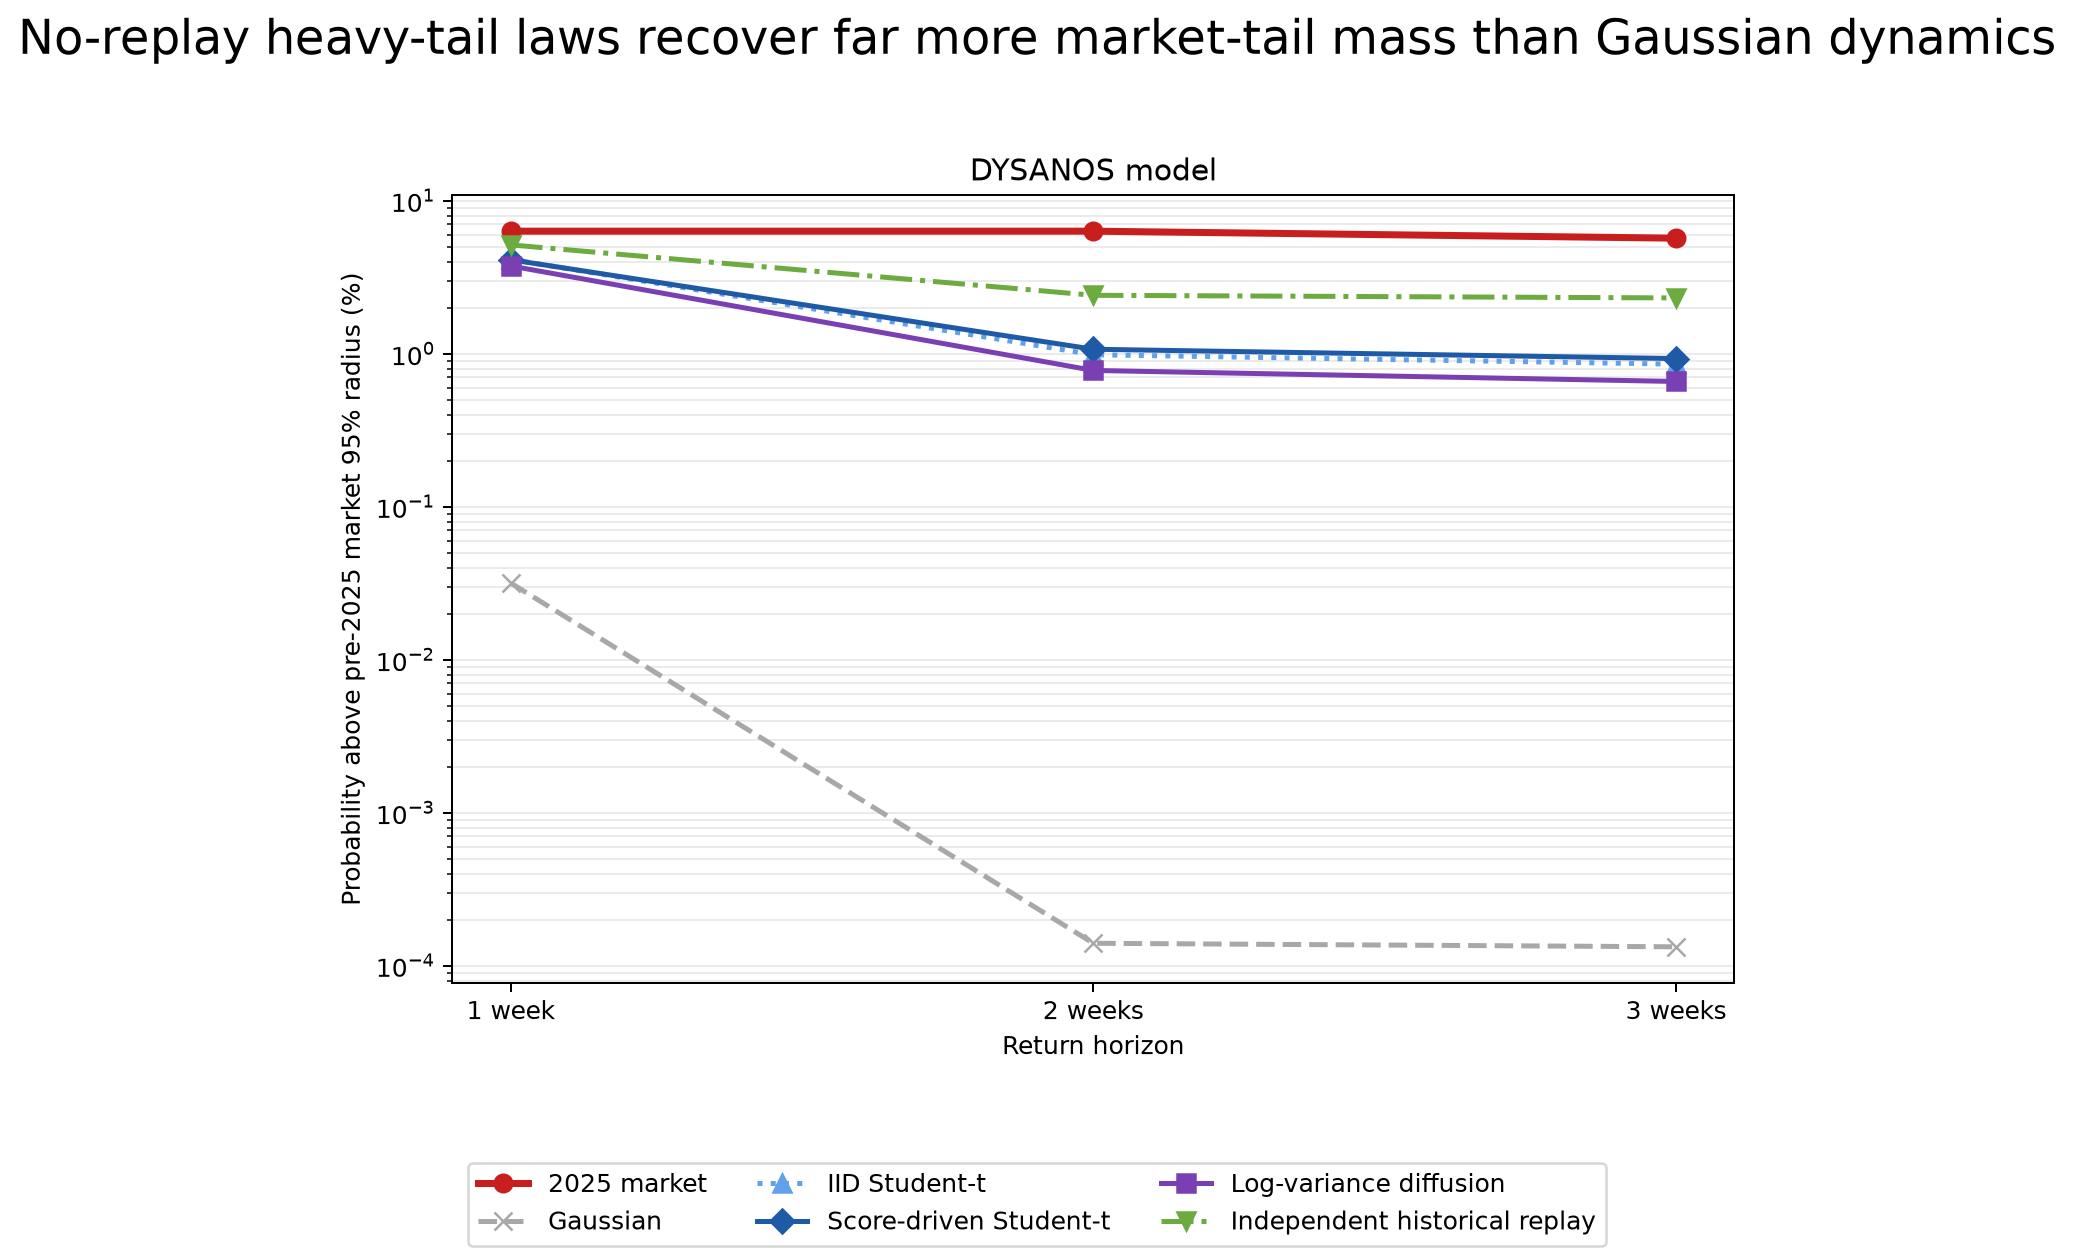
\includegraphics[width=\textwidth]{generated/presentation_tail_exceedance.png}
  \caption{Probability of exceeding the pre-2025 market 95\%
  normalized-radius threshold, on a logarithmic scale.  Both no-replay
  heavy-tail laws recover orders of magnitude more tail mass than Gaussian
  innovations but remain too light at two and three weeks.}
  \label{fig:tail-exceedance}
\end{figure}

The no-replay diffusion is therefore a meaningful improvement, not a complete
tail model.  It also produces squared-radius serial correlations of 0.206 and
0.116, compared with 0.133 and 0.091 in the weekly and daily+weekly market
histories; Gaussian and IID laws have zero population correlation.  The 2025
sample is small and overlapping: 15-origin circular-block bootstrap 95\%
intervals for the market exceedance rates are approximately 0.6--14.6\%
across the six geometry/horizon cells.  Differences of a percentage point
should therefore not be over-interpreted.  Independent historical replay is
still closest in marginal tail mass, while the diffusion is a fully
parametric generator with fresh support and explicit persistence.

\subsection{Chronological surface-path comparison}
\label{sec:path-realism}

Horizon radii test the latent innovation law but do not directly test paths
of decoded option prices.  We therefore form every available sequence of four
fitted market-state surfaces separated by one full trading week, giving three
consecutive weekly changes.  Here ``observed'' means the date-specific latent
state fitted to that day's irregular quote book and then passed through the
common SANOS decoder; it is not a second interpolation of the raw quotes.
Every candidate simulator starts from that fitted surface at the same origin
date.  Its path features are changes in normalized call prices on
the Cartesian panel of target locations
\[
  T\in\{1,5,10,20,40,70\}\text{ business days},
  \qquad
  K/S\in\{0.85,0.90,0.95,1.00,1.05,1.10,1.15\}.
\]
Each target expiry is mapped to the closest distinct model expiry.  The
daily+weekly geometry therefore has $3\times6\times7=126$ features; in the
weekly geometry the 1D and 5D targets both map to 5D, leaving
$3\times5\times7=105$.  Coordinates are centered and scaled using pre-2025
observed paths only.

For this path-level test, the historical comparator replays an entire
pre-2025 three-week sequence of fitted residuals, rather than drawing its
three weekly residuals independently.  It is therefore a deliberately strong
finite-sample benchmark that preserves short-run clustering, but it is not a
new parametric law and cannot generate innovations outside the stored blocks.

We report the standardized energy distance and an unbiased Gaussian-kernel
maximum mean discrepancy (MMD) between observed and simulated 2025 paths.
For the null distribution, entire paired chronological blocks of 15 origin
dates swap their observed/simulated labels; the block length matches the
three-week feature horizon and retains most overlap-induced dependence.
1,999 random block swaps give a Monte Carlo $p$-value with minimum positive
resolution $0.0005$.

The 2025 split is a chronological holdout for fitting any auxiliary tail law,
constructing a historical-residual pool, and estimating the feature
standardization.  The shared affine decoder and the baseline Gaussian AR law
are nevertheless taken from the all-history checkpoint.  The path comparison
is therefore a holdout diagnostic for the innovation-law extensions
conditional on the learned representation, not a fully frozen pre-2025 model
forecast.

Table~\ref{tab:path-realism} reports 144 paired 2025 paths for each geometry.
The $p$-value is the block-swap test for MMD; energy distance is reported as a
second scale-sensitive discrepancy.  None of the five candidates is rejected
at 5\%.  This is evidence against a gross path-distribution failure, but not a
ranking theorem: IID Student-$t$ has the smallest weekly energy distance,
whereas Gaussian has the smallest daily+weekly energy and MMD.  The
log-variance diffusion remains statistically plausible while improving the
separate tail and persistence diagnostics above.

\begin{table}[H]
\centering
\small
\begin{tabular}{lrrrrrr}
\toprule
& \multicolumn{3}{c}{Weekly} & \multicolumn{3}{c}{Daily+weekly}\\
\cmidrule(lr){2-4}\cmidrule(lr){5-7}
Innovation law & Energy & $10^3\!\times$MMD$^2$ & $p$ & Energy & $10^3\!\times$MMD$^2$ & $p$\\
\midrule
Gaussian & 0.572 & 4.602 & 0.550 & 0.810 & 1.594 & 0.704\\
IID Student-$t$ & 0.540 & 5.016 & 0.344 & 0.854 & 3.788 & 0.457\\
Score-driven Student-$t$ & 0.569 & 4.389 & 0.225 & 0.838 & 3.786 & 0.416\\
Log-variance diffusion & 0.606 & 5.476 & 0.378 & 0.854 & 3.480 & 0.415\\
Historical block replay & 0.592 & 6.671 & 0.328 & 0.857 & 6.968 & 0.345\\
\bottomrule
\end{tabular}
\caption{Chronological decoded-surface path diagnostics on 144 paired 2025
origins.  Each path contains three consecutive weekly changes; $p$ is based
on 1,999 paired 15-origin block swaps.}
\label{tab:path-realism}
\end{table}

\subsection{Stability diagnostics}

\begin{table}[H]
\centering
\begin{tabular}{lrr}
\toprule
Statistic & Weekly & Daily+weekly\\
\midrule
State dimension & 200 & 200\\
Dates & 891 & 891\\
Exact 1W innovations & 861 & 861\\
$\rho(A)$ & 0.9577 & 0.9561\\
Slowest-mode half-life & 16.1 weeks & 15.4 weeks\\
Minimum real eigenvalue of $\kappa$ & 0.0432 & 0.0449\\
Invariant covariance condition number & 3.51 & 3.64\\
Invariant covariance effective rank & 196.5 & 196.4\\
\bottomrule
\end{tabular}
\caption{Fitted state-law diagnostics.}
\label{tab:stability}
\end{table}

Both laws are stable and retain almost full effective rank in state space.  A
simulator can therefore start from an observed state or draw
$h_0\sim\mathcal N(m,P)$ when a stationary initialization is appropriate.

\subsection{Conditional front-expiry spot block}


\begin{remark}[Normalization with forwards and discount factors]
\label{rem:driftreturnsa}
If the market has discount factors
$\bm{DF}_t(T)=\exp(-R_t(T))$ and forwards
$\bm{F}_t(T)=\bm{S}_t\exp(R_t(T)-D_t(T))$, the normalized one-step
log-spot return is
\[
  \Delta s_{t+1}
  =\log\bm{S}_{t+1}
   -\log\!\bigl(\bm{DF}_t(\Delta t)\bm{F}_t(\Delta t)\bigr)
  =\log\bm{S}_{t+1}-\log\bm{S}_t+D_t(\Delta t).
\]
Option prices require no further drift adjustment here because the input
surface has already been expressed in forward- and discount-normalized units.
\end{remark}

The normalized option surface can be simulated autonomously.  Cash spot is
attached through the front-expiry SANOS distribution while preserving its
observed contemporaneous dependence with surface innovations.  Let
$F_t^1$ denote the CDF obtained from the first decoded SANOS density, including
the lognormal backbone, and let $z_{t+1}$ be the whitened one-session state
innovation.  Each observed gross spot return is transformed to its front-law
Gaussian score
\begin{equation}
  g_{t+1}=\Phi^{-1}\!\left[
    F_t^1\!\left(\frac{S_{t+1}}{S_t}\right)
  \right].
  \label{eq:front-spot-score}
\end{equation}
On transitions preceding the evaluation window, we estimate a ridge loading
$b$ by regressing the standardized $g_{t+1}$ on $z_{t+1}$.  Its penalty is
selected by time-ordered validation.  If $\sigma_\perp$ is the fitted residual
standard deviation, a joint scenario uses independent standard normals
$Z\in\mathbb R^{200}$ and $\epsilon\in\mathbb R$ and sets
\begin{equation}
  G=\frac{b'Z+\sigma_\perp\epsilon}
          {\sqrt{b'b+\sigma_\perp^2}},
  \qquad
  \frac{S_{t+1}}{S_t}
    =(F_t^1)^{-1}\!\left(\Phi(G)\right).
  \label{eq:spot-block}
\end{equation}
The same $Z$ drives the next surface state.  Consequently the spot draw has
the current front-expiry marginal and the fitted spot--surface copula rather
than being independent of the surface shock.  For each date we tabulate
$F_t^1$ on a fine log-return grid and invert it with a monotone PCHIP spline.
This is an interpolation of the quantile function; it avoids a separate
root solve for every scenario without sacrificing monotonicity.  Log-spot
itself is not part of the invariant surface state.

Because $F_t^1$ is the option-implied risk-neutral front-expiry marginal, this
construction does not estimate or add a physical spot drift.  Its first moment
is fixed by the observed front forward (and equals one in forward-normalized
units), so spot carries the one-step risk-neutral drift implied by market
carry.  The fitted copula changes only the dependence between spot and surface
innovations; it does not change the spot marginal or its drift.

\subsection{Decoded implied-volatility geometry}
\label{sec:pca}

Although $h_t$ has 200 coordinates, decoded implied-volatility variation is
much lower-dimensional.  We differentiate the affine SANOS decoder at the
invariant mean and combine its Jacobian with $P$.  The resulting PCs are
directions in decoded implied-volatility space, not the learned state
coordinates.

\begin{table}[H]
\centering
\begin{tabular}{lrr}
\toprule
Cumulative decoded-IV variance & Weekly & Daily+weekly\\
\midrule
PC1 & 74.85\% & 77.68\%\\
PC1--2 & 86.97\% & 86.98\%\\
PC1--4 & 95.63\% & 94.50\%\\
PC1--8 & 99.46\% & 99.39\%\\
\bottomrule
\end{tabular}
\caption{Decoded implied-volatility variance under the invariant state law.}
\label{tab:decoded-pca}
\end{table}

Figure~\ref{fig:pca-spectrum} gives the full leading spectrum.  PC1 is a
nearly parallel volatility-level move and explains 74.85\% of weekly decoded
variance and 77.68\% of daily+weekly decoded variance.  Four decoded-IV
factors explain 95.63\% and 94.50\%, respectively.  This does not imply that
four latent coordinates would fit the quote book: the PCA is performed
\emph{after} the 200-state model has been passed through the nonlinear SANOS
decoder and weighted by its invariant covariance.

\begin{figure}[p]
  \centering
  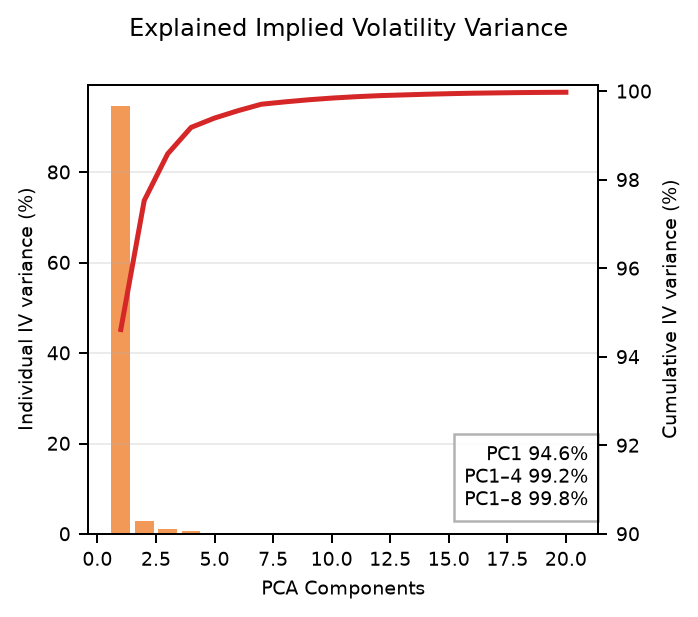
\includegraphics[width=\textwidth]{generated/presentation_decoded_iv_pca_spectrum.png}
  \caption{Variance explained by PCA of decoded implied-volatility levels
  under the fitted invariant state laws.  The 200 affine coordinates are not
  themselves these PCs.}
  \label{fig:pca-spectrum}
\end{figure}

The invariant means in Figure~\ref{fig:base-vol-surfaces} are the natural
``base volatility'' surfaces of the two statistical models.  Their broad
term-structure and skew geometry is similar.  The difference is concentrated
at the front: the daily+weekly model has four additional expiry slices with
independent DLV and forward-volatility coordinates, whereas the weekly model
extrapolates from 5D.

\begin{figure}[p]
  \centering
  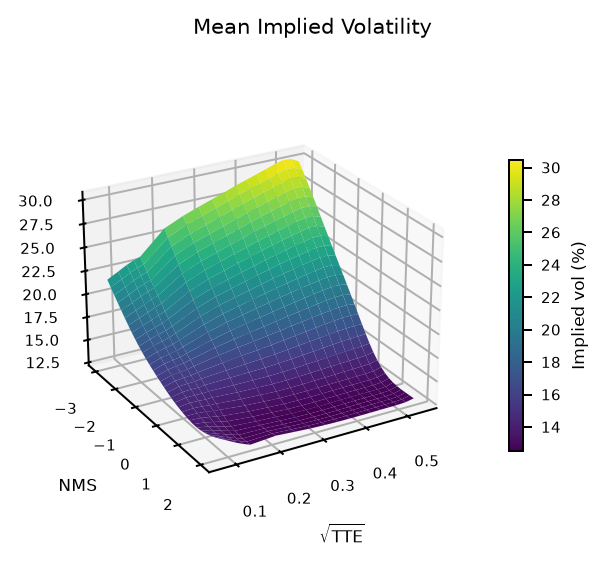
\includegraphics[width=\textwidth]{generated/presentation_invariant_mean_iv_surfaces.png}
  \caption{Base implied-volatility surfaces, obtained by evaluating each
  affine SANOS decoder at the invariant state mean.  Axes are square-root
  time-to-expiry, normalized moneyness, and annualized implied volatility.}
  \label{fig:base-vol-surfaces}
\end{figure}

Figures~\ref{fig:weekly-pca-factors} and
\ref{fig:daily-weekly-pca-factors} show the first eight eigensurfaces.  Each
panel is one invariant standard deviation and has its own vertical scale; PCA
signs are arbitrary.  PC1 is the global level.  PC2 is primarily a broad
skew/term-structure rotation, while PC3 couples skew and maturity.  Higher
modes become increasingly localized.  The daily+weekly model places visibly
more of those localized modes at 1D--4D, which is precisely the flexibility
needed to fit the front-end quote book.

\clearpage
\begin{landscape}
\begin{figure}[p]
  \centering
  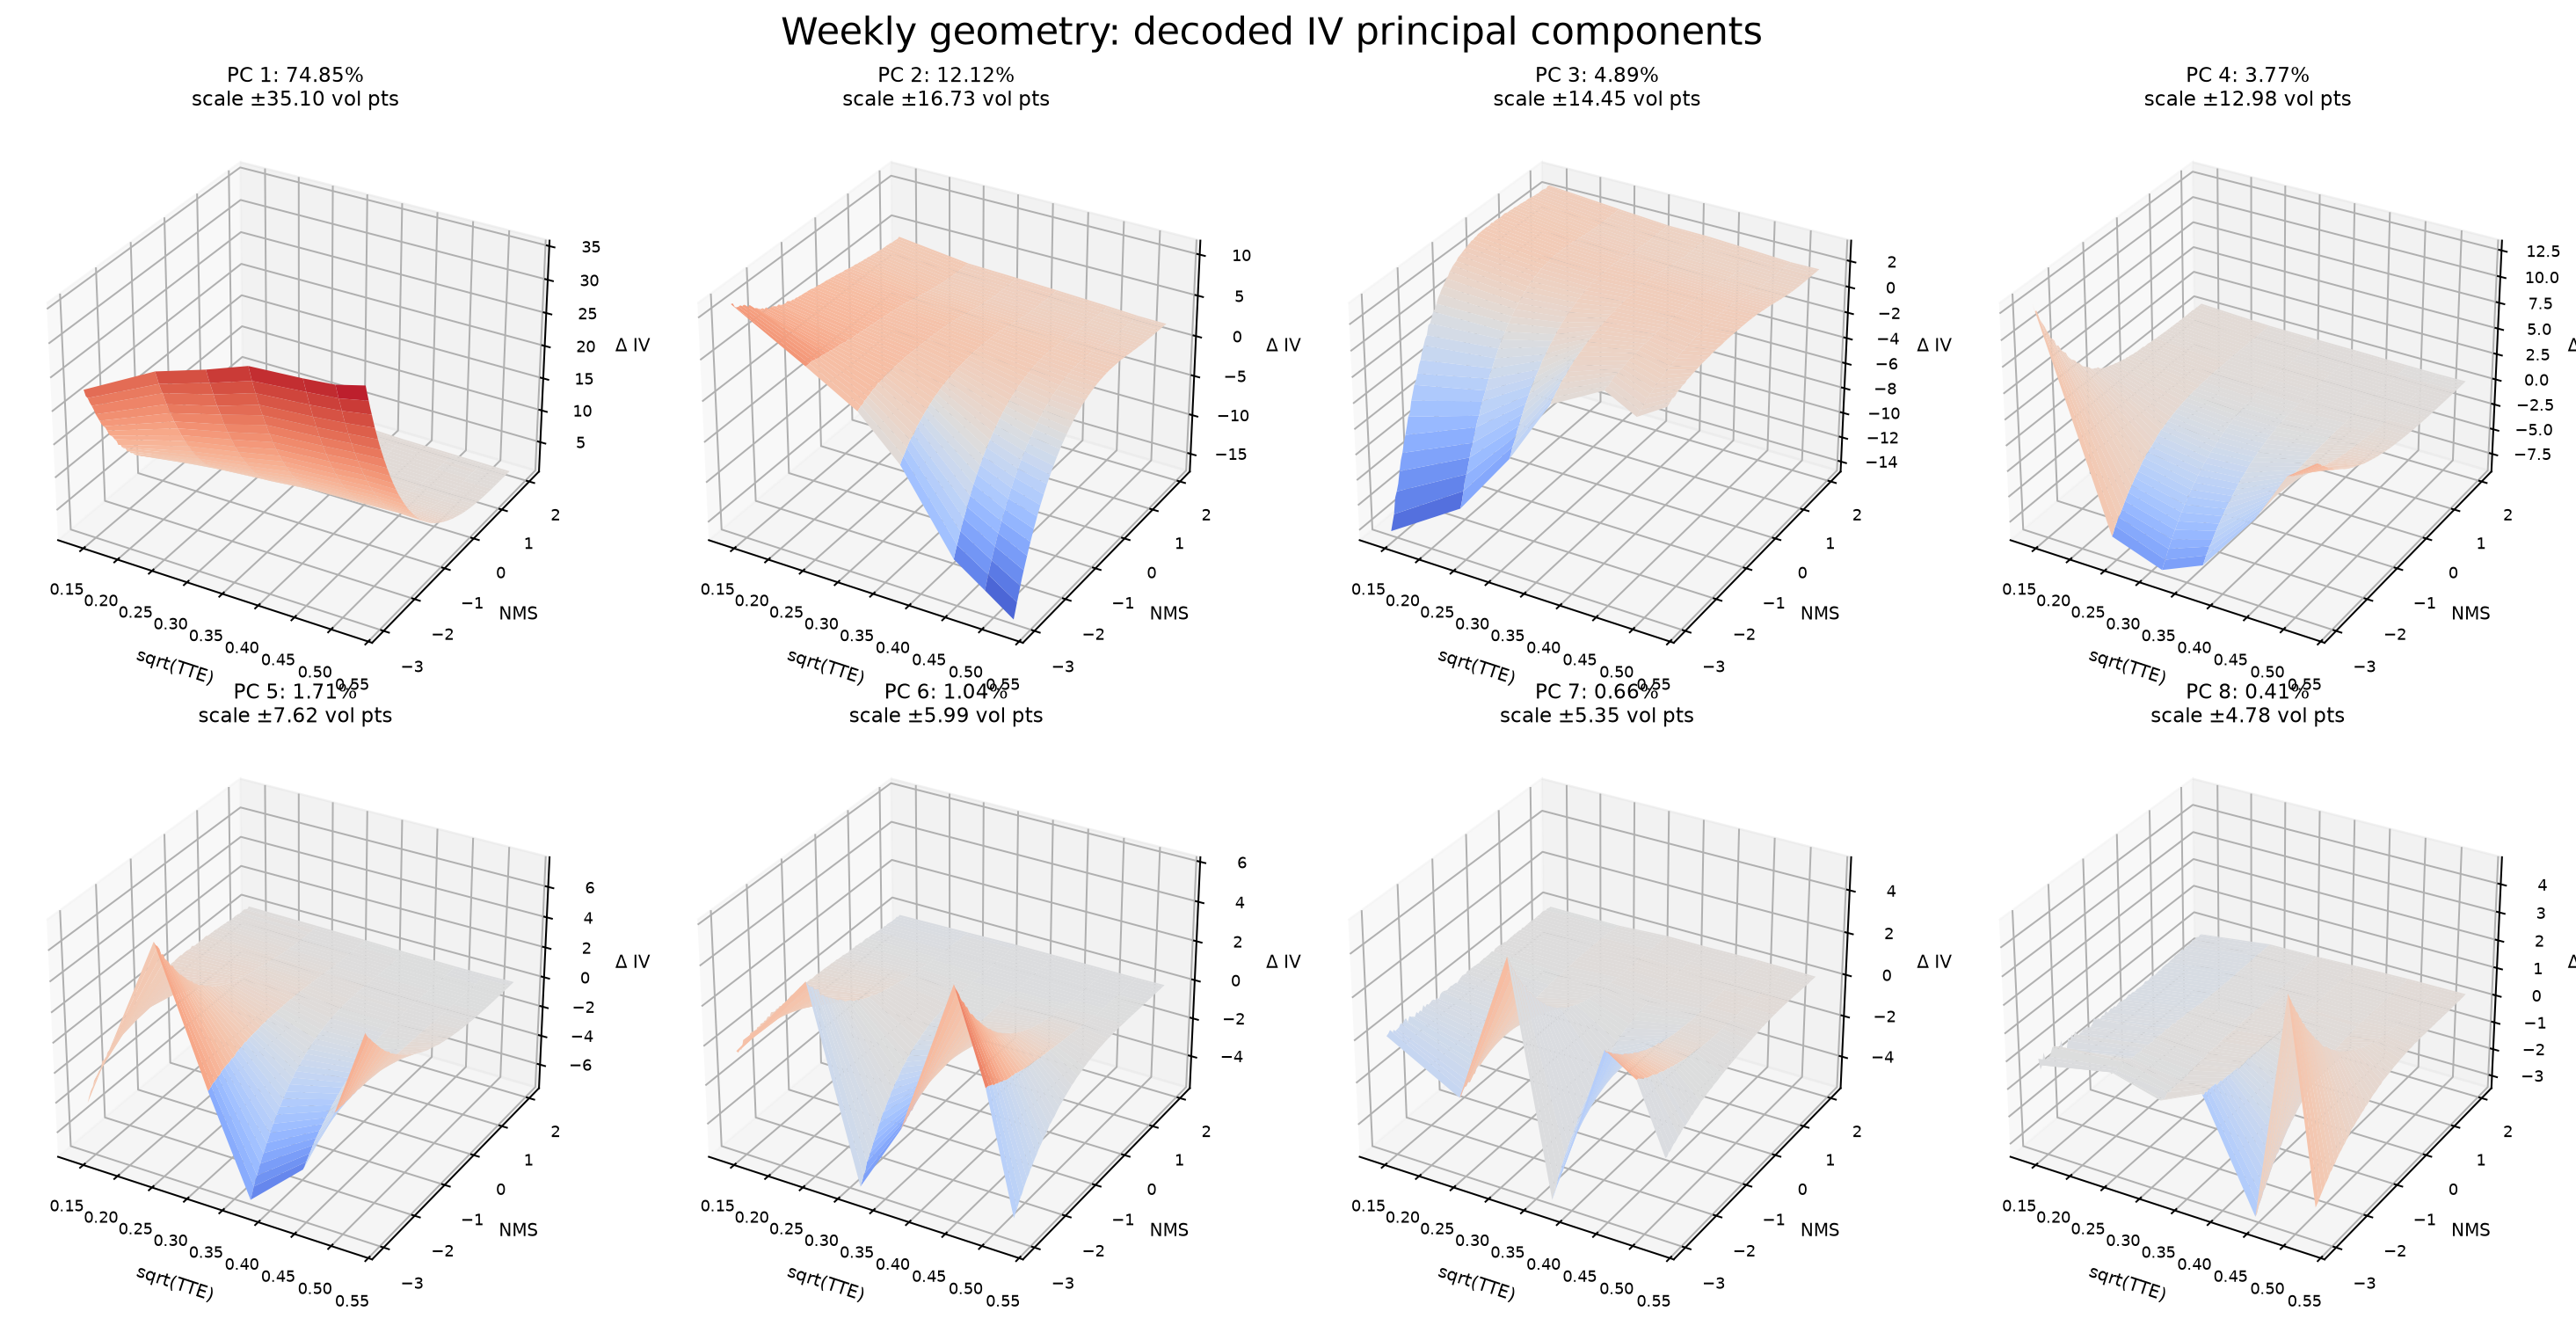
\includegraphics[width=\linewidth]{generated/presentation_weekly_iv_pca_factors.png}
  \caption{Weekly geometry: decoded implied-volatility PCs 1--8 at one
  invariant standard deviation.  The title of each panel reports explained
  variance and the panel-specific move in volatility points.}
  \label{fig:weekly-pca-factors}
\end{figure}
\end{landscape}
\clearpage

\begin{landscape}
\begin{figure}[p]
  \centering
  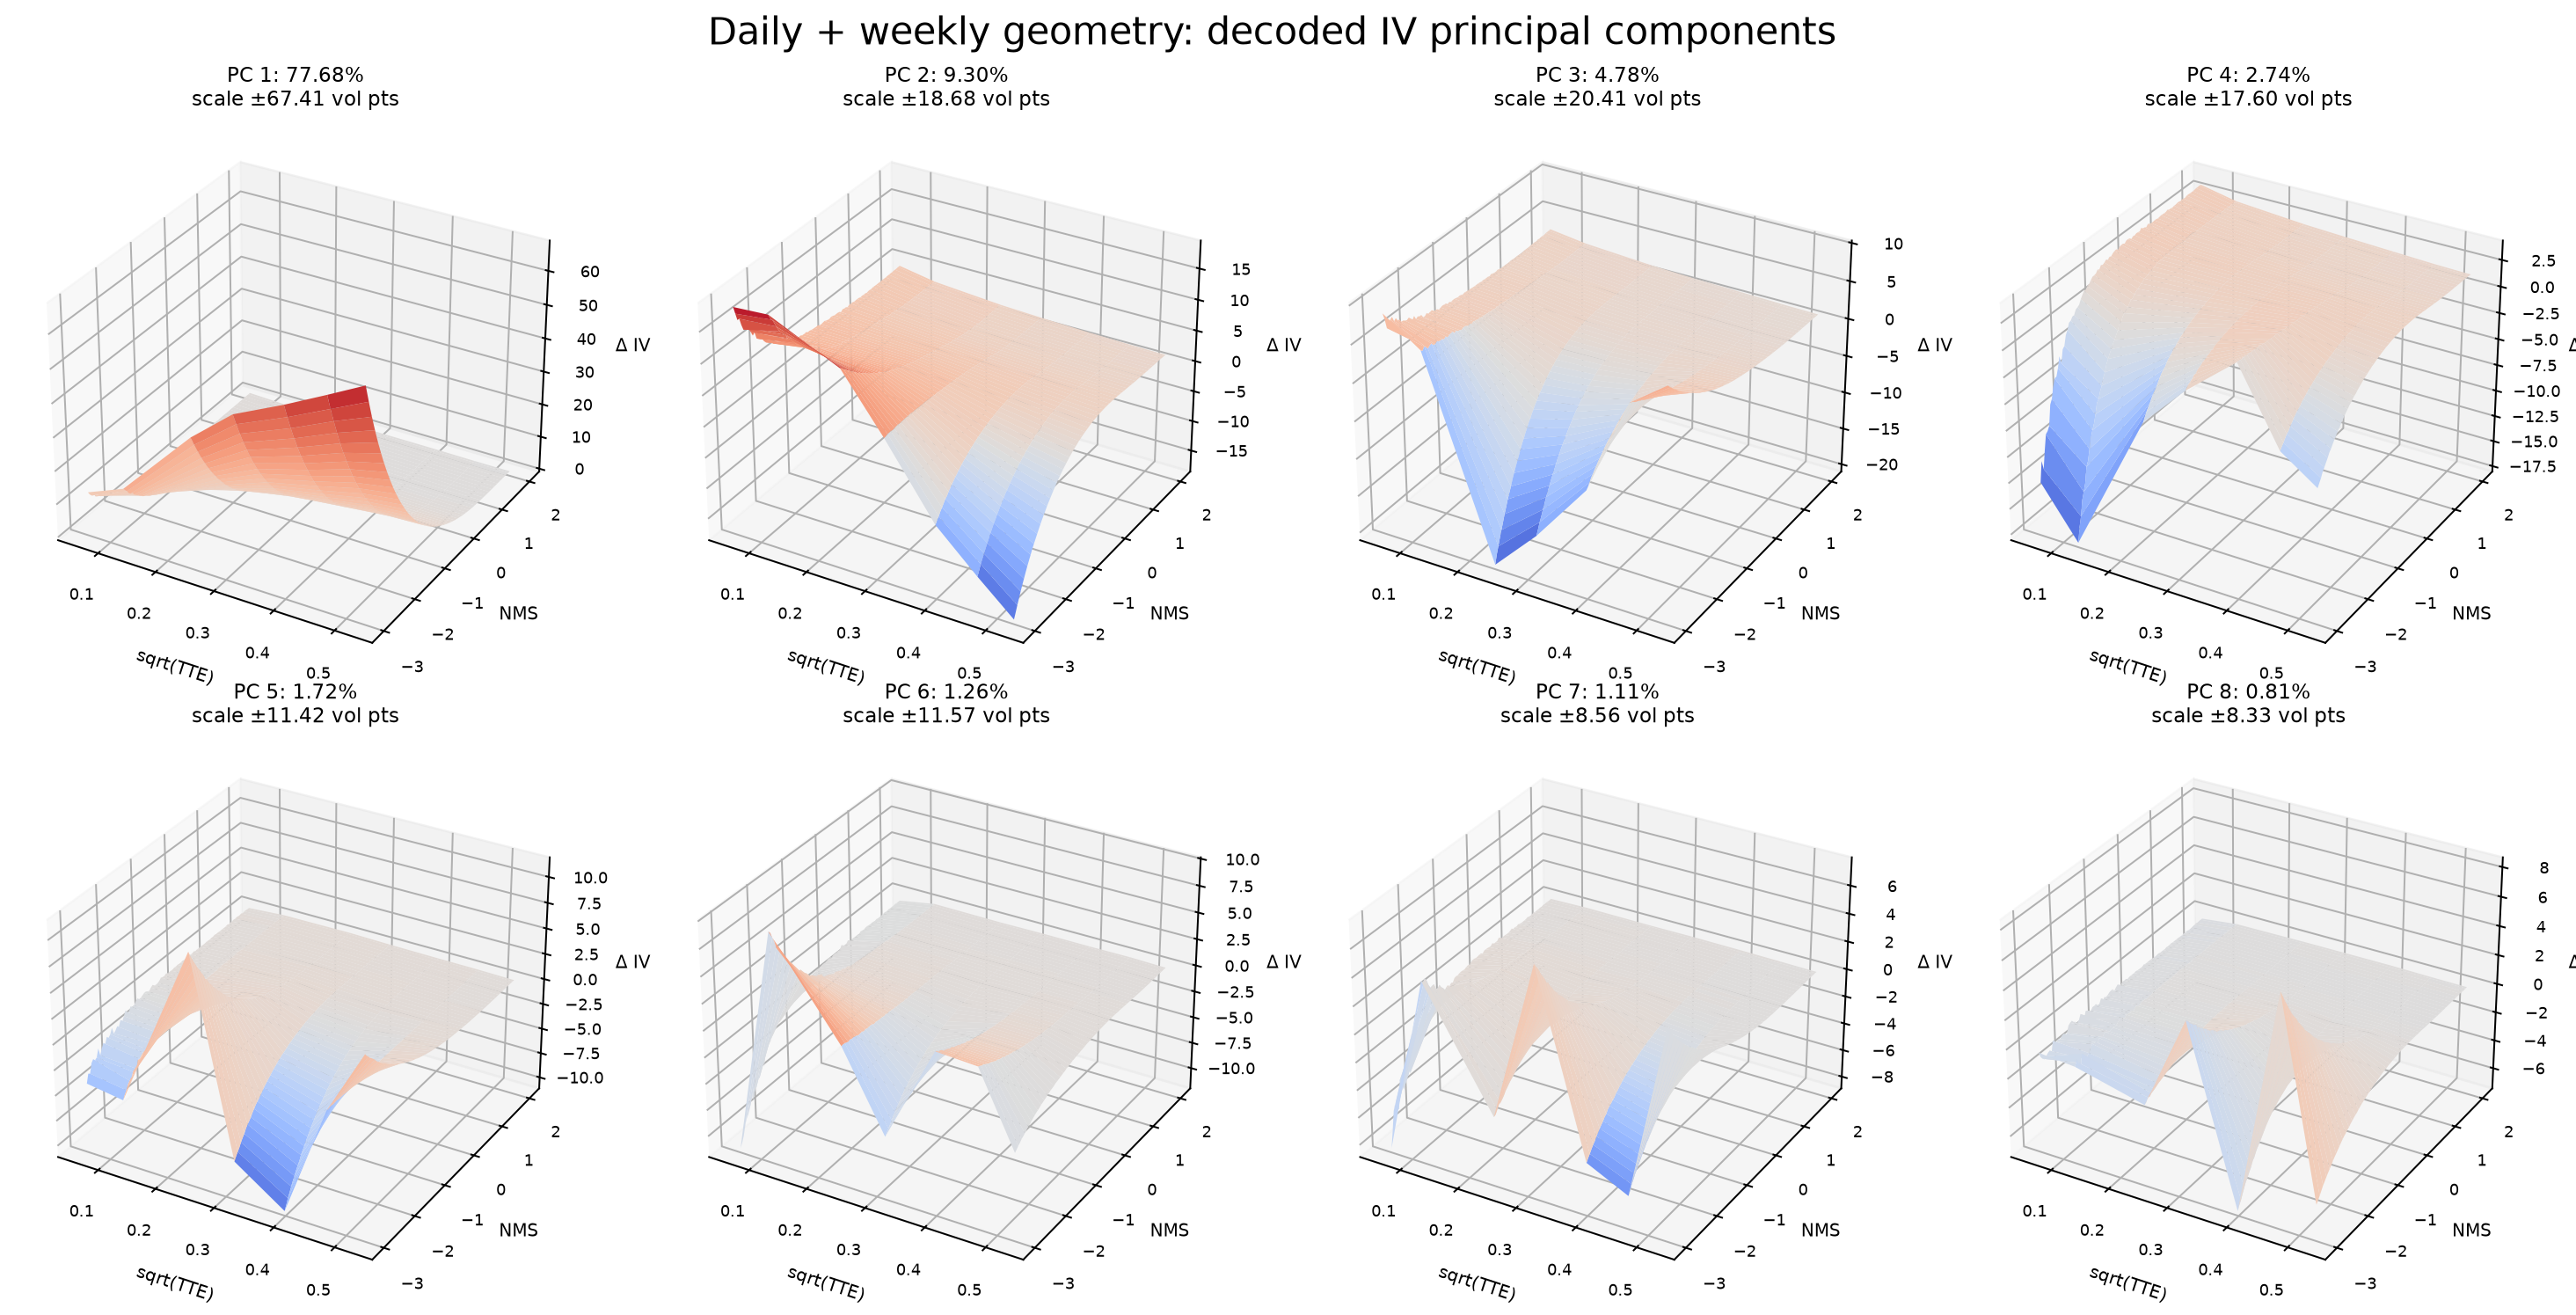
\includegraphics[width=\linewidth]{generated/presentation_daily_weekly_iv_pca_factors.png}
  \caption{Daily+weekly geometry: decoded implied-volatility PCs 1--8 at one
  invariant standard deviation.  Additional front-end modes appear because
  1D--4D are explicit model expiries.}
  \label{fig:daily-weekly-pca-factors}
\end{figure}
\end{landscape}
\clearpage

\subsubsection{Invariant-distribution visualization}

The PCA summarizes local covariance at the invariant mean; complete nonlinear
decodes verify what that covariance produces as a surface distribution.
Figure~\ref{fig:invariant-atm-draws} shows six independent draws from each
fitted $\mathcal N(m,P)$ state law.  The weekly model's sub-5D ATM term
structure is visibly constrained by extrapolation from its first node.  The
daily+weekly model can generate sharp but still statically admissible
front-end dislocations.

\begin{figure}[H]
  \centering
  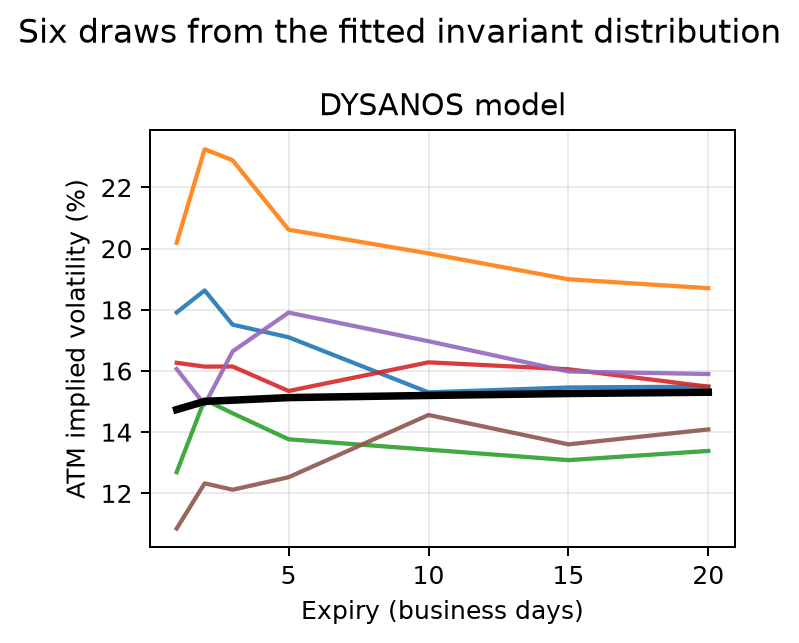
\includegraphics[width=\textwidth]{generated/presentation_invariant_atm_draws.png}
  \caption{ATM implied-volatility term structures from six independent
  invariant-state draws for each model.  Black is the invariant-mean decode.
  These are stationary cross-sectional samples, not consecutive time steps.}
  \label{fig:invariant-atm-draws}
\end{figure}

Figure~\ref{fig:invariant-surface-draws} uses the same 200-dimensional
standard-normal seed for both models, mapped through each model's own
invariant covariance and decoder.  It provides a controlled visual comparison
of complete draws: their long-end shapes remain broadly comparable, while the
daily+weekly surface has materially richer short-end geometry.

\begin{figure}[H]
  \centering
  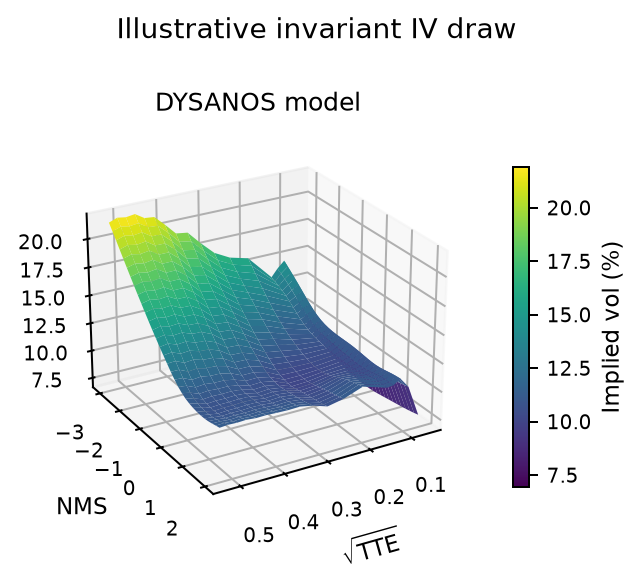
\includegraphics[width=\textwidth]{generated/presentation_invariant_surface_draws.png}
  \caption{Paired complete invariant-state surface draws.  A common standard
  normal seed is transformed by each fitted invariant covariance before being
  decoded by the corresponding affine SANOS model.}
  \label{fig:invariant-surface-draws}
\end{figure}
\clearpage

\subsection{Simulation algorithm}
\label{sec:simulation}

The statistical DYSANOS simulator is summarized as follows.
\begin{enumerate}
  \item Choose the daily+weekly geometry and initialize $h_0$ from an observed
        date or from the invariant state distribution.
  \item Propagate the state with the exact Gaussian transition
        \eqref{eq:exact-transition}, or use the no-replay log-variance
        diffusion \eqref{eq:sv-innovation}--\eqref{eq:sv-logvariance} when
        persistent tails are required.  Historical innovation replay remains
        a non-parametric weekly benchmark.
  \item If cash prices are required, propagate $s_t$ conditionally using
        \eqref{eq:spot-block}.
  \item Form $u_t=b+B h_t$, map it to bounded SANOS parameters through
        \eqref{eq:defDLVdsq} and \eqref{eq:totalW}, and apply
        the density recursion of Section~\ref{sec:mlsanos}.
  \item Evaluate $C_t(T,K)$ at any desired strike and expiry.  For a fixed
        cash contract $(\tau,k)$ use $T=\tau-t$ and $K=k/S_t$.
\end{enumerate}

The AR transition and SANOS decoder serve different roles.  Stability of the
first supplies a coherent long-run statistical state process; the second
guarantees a valid option cross-section for every realized state.  The
combination is what we mean by consistent $\P$-simulation in this paper.

\subsection{Fixed-sample to-expiry entropy projection}
\label{sec:fixed-sample-entropy}

As a finite-sample diagnostic, we ask whether the simulated law can be
reweighted so that a rolling option book has no expected return outside an
explicit transaction-cost band.  Both experiments use one historical initial
state (25 October 2023) and $N=1{,}000{,}000$ antithetic simulated paths.  Each
option has a fixed cash strike set on its entry date and is held to its
terminal payoff.  The admissible expected-return band is 1bp for spot and
10bp for each option, representing symmetric entry costs.

We considered two nested books.  The pilot book contains spot and, for each
of 5D, 10D, 15D, and 20D, a call struck at $K/S_t=0.99$, an ATM call, and a
put struck at $K/S_t=1.01$.  Repeating these 13 instruments on each of 25
entry dates gives $25\times13=325$ return coordinates.

The expanded book replaces those three options by 11 normalized-moneyness
coordinates at every expiry,
\begin{equation}
  z\in\{-1.5,-1.3,-1.1,-0.9,-0.7,-0.5,-0.3,-0.1,
          0.1,0.3,0.5\}.
  \label{eq:entropy-book-nms}
\end{equation}
At entry time $t$, normalized moneyness $z$ is converted to the cash strike
\begin{equation}
  K=S_t\exp\!\bigl(z\,\nu_t(T)\bigr),\qquad
  \nu_t(T)=\sqrt{\frac{\sigma_{t,\epsilon}^2\epsilon+
                           \widetilde W_t(T)^2}
                           {1+\epsilon}},
  \label{eq:entropy-book-strike}
\end{equation}
where $\widetilde W_t(T)$ is the strike-grid total volatility from
\eqref{eq:totalW},
$\sigma_{t,\epsilon}=\widetilde W_t(\hat T^1)/\sqrt{\hat T^1}$, and
$\epsilon$ is the canonical small-time regularization.  Negative-$z$
contracts are ITM calls and positive-$z$ contracts are ITM puts.  The grid in
\eqref{eq:entropy-book-nms} deliberately does not contain zero, so this
expanded book has no ATM option.  With spot and $4\times11$ options at each
entry date it has $25\times45=1{,}125$ return coordinates.

Let $R_n\in\mathbb R^d$ be the return vector on path $n$, where
$d\in\{325,1{,}125\}$, let $c\in\mathbb R_+^d$ be the cost band, and let
$w_n$ denote an empirical
density relative to the uniformly weighted simulation sample.  We solve the
convex information projection
\begin{equation}
\begin{aligned}
  \min_{w_1,\ldots,w_N>0}\quad
    &\frac1N\sum_{n=1}^N w_n\log w_n,\\
  \text{subject to}\quad
    &\frac1N\sum_{n=1}^N w_n=1,\\
    &-c\ \leq\ \frac1N\sum_{n=1}^N w_nR_n\ \leq\ c.
\end{aligned}
\label{eq:fixed-sample-entropy}
\end{equation}
The dual is a signed entropic OCE objective.  We solve it with an active-set
method and streamed log-sum-exp evaluations, so the complete million-path
return matrix need not be copied into the optimizer.

\begin{table}[H]
\centering
\small
\begin{tabular}{lrr}
\toprule
Diagnostic & Three-option pilot & 11-option NMS book\\
\midrule
Paths & 1,000,000 & 1,000,000\\
Options per expiry & 3 & 11\\
Return coordinates & 325 & 1,125\\
Active coordinates & 207 & 336\\
Relative entropy $N^{-1}\sum_n w_n\log w_n$
  & 0.0619141 & 0.1130914\\
Effective sample size & 877,973 (87.80\%) & 765,493 (76.55\%)\\
Minimum density weight & 0.00880 & 0.00286\\
Maximum density weight & 36.42 & 84.17\\
Zero density weights & 0 & 0\\
Maximum cost-band violation & $8.45\times10^{-8}$ & $3.15\times10^{-8}$\\
Maximum KKT residual & $8.45\times10^{-8}$ & $3.53\times10^{-8}$\\
Primal--dual gap & $7.14\times10^{-9}$ & $3.37\times10^{-9}$\\
\bottomrule
\end{tabular}
\caption{In-sample convex entropy projection for rolling to-expiry returns.
Residuals are in return units.  The maximum cost-band violations are
0.000845bp and 0.000315bp, respectively.}
\label{tab:fixed-sample-entropy}
\end{table}

All fitted weights are strictly positive.  The expanded book retains 76.55\%
of the original effective sample size despite imposing 1,125 moment bands.
For both books the optimizer terminated during its final line search rather
than returning its strict success flag.  The independently recomputed primal,
KKT, and primal--dual residuals in Table~\ref{tab:fixed-sample-entropy} show
that the economically relevant cost-band constraints are nevertheless
satisfied to substantially less than one thousandth of a basis point.

This is deliberately an \emph{in-sample, unconditional} statement.  The
weights solve empirical moment constraints for this initial state and this
fixed path population.  They do not prove the existence of a single
state-conditional transition density, do not constitute an out-of-sample
forecast, and do not alter the statistical dynamics used elsewhere in the
paper.  The experiment nevertheless establishes that the selected finite
book is compatible with a well-conditioned, absolutely continuous empirical
reweighting when contracts are evaluated to expiry.

Section~\ref{sec:risk-neutral} builds on this reweighting with a genuinely
state-conditional construction.

\subsection{Scope and limitations}

The 80.92\% market-fit figure is computed on the population used to estimate
the final all-history model.  It is not a claim of 80\% future forecast
coverage.  A formal forecasting study should freeze the decoder and dynamics
before the evaluation period.

The Gaussian state law severely understates tail frequency.  The no-replay
log-variance diffusion improves likelihood, tail mass, and serial-tail
dependence, but still underproduces two- and three-week extremes.  Historical
innovation replay is closer in marginal tail mass, while the path-level tests
have only 144 overlapping 2025 origins and do not distinguish the candidates
sharply.  A richer multiscale or regime-dependent volatility law is the most
direct next extension.

Finally, static arbitrage-freedom is a property of each decoded surface.  It
does not by itself impose restrictions on expected returns of fixed contracts
through simulated time.  The fixed-sample entropy projection in
Section~\ref{sec:fixed-sample-entropy} is an unconditional diagnostic for one
finite simulated population, not an additional dynamic pricing assertion.
Section~\ref{sec:risk-neutral} reports a first, explicitly reduced attempt at
a genuine dynamic construction.

\section{Risk-Neutral DYSANOS}
\label{sec:risk-neutral}

Static arbitrage-freedom of each decoded surface does not by itself impose a
martingale restriction on the returns of fixed contracts through simulated
time (Section~\ref{sec:fixed-sample-entropy}).  We here report a first,
deliberately reduced demonstration that a genuine \emph{near-martingale}
measure can nevertheless be constructed for a subset of tradable contracts by
applying the Deep Hedging drift-removal method of
\cite{removedrift,removelong} directly to simulated DYSANOS paths.  We do not
claim risk-neutrality of the full surface; extending the construction to
\emph{all} options is ongoing work.

\subsection{Universe and pre-conditioning}
\label{sec:risk-neutral-universe}

We trade spot and, at each of 25 fixed trading dates, floating options at the
four expiries $5D,10D,15D,20D$ struck on the same 11-point normalized-moneyness
grid~\eqref{eq:entropy-book-nms} via~\eqref{eq:entropy-book-strike}; once
entered, each option is a fixed contract $(\tau,k)$ held to its own expiry.
This is the same $44+1=45$-dimensional ``expanded book'' and the same
$N=1{,}000{,}000$ fixed simulated paths used for the 11-option NMS entropy
projection in Table~\ref{tab:fixed-sample-entropy}.  Writing $C_t^i$ for the
entry price and $V_t^i$ for the (spot or option) expiry value of instrument
$i$, returns are expressed as fractional gains,
\begin{equation}
  R_t^i=\frac{V_t^i}{C_t^i}-1,
  \qquad i=1,\ldots,45,
  \label{eq:rn-returns}
\end{equation}
and entry costs are $c^{\mathrm{spot}}=1$bp and $c^{\mathrm{opt}}=10$bp of
traded dollar notional.\footnote{For numerical stability the Deep Hedging
training in this section uses one tenth of these costs.}

As a pre-condition we reuse the convex projection~\eqref{eq:fixed-sample-entropy}:
its solution $w$ defines a reweighted measure $\P^w$ via
$d\P^w/d\P|_{\{\omega_n\}}=w_n$, under which every return in the book has zero
unconditional drift up to its cost band,
$\bigl|\E^{\P^w}[R_t^i]\bigr|\leq c^i$.

\subsection{A near-martingale measure via Deep Hedging}

Let $u$ be a smooth, strictly increasing, concave utility with
$u(0)=0$, $u'(0)=1$, $\lim_{x\to-\infty}u'(x)=\infty$, $\lim_{x\to\infty}u'(x)=0$;
our experiments use the entropy utility $u(x)=(1-e^{-\lambda x})/\lambda$.
Following~\cite{OCE}, the associated OCE monetary utility
\begin{equation}
  U(X):=\sup_{y\in\R}\;\E^{w}\bigl[u(y+X)-y\bigr]
  \label{eq:rn-oce}
\end{equation}
is increasing, concave, and cash-invariant,
$U(X+c)=U(X)+c$ for $c\in\R$; for the entropy utility it reduces to the
entropic certainty equivalent
$U(X)=-\lambda^{-1}\log\E^w[\exp(-\lambda X)]$.

Trading actions are parameterized directly on the state $x_t=(s_t,h_t)$
already used for $\P$-simulation (Section~\ref{sec:simulation}),
\begin{equation}
  a_\theta(x_t)=W_\theta x_t+F_\theta(x_t)+b_\theta\ \in\R^{45},
  \label{eq:rn-action}
\end{equation}
where $W_\theta$ is a matrix, $b_\theta$ a vector, and $F_\theta$ a
three-layer SeLU network with 128 inner nodes per layer.

We solve the empty-portfolio Deep Hedging problem under $\P^w$,
\begin{equation}
  \sup_{\theta,\,y\in\R}\;
  \E^{\P^w}\Bigl[
    u\Bigl(y+\textstyle\sum_t a_\theta(x_t)'R_t-\bigl|a_\theta(x_t)\bigr|'c\Bigr)-y
  \Bigr]
  \;\longrightarrow\;\theta^*,y^*,
  \label{eq:rn-deephedge}
\end{equation}
and define the candidate density
\begin{equation}
  \frac{d\Q}{d\P^w}:=
  u'\Bigl(y^*+\textstyle\sum_t a_{\theta^*}(x_t)'R_t-\bigl|a_{\theta^*}(x_t)\bigr|'c\Bigr).
  \label{eq:rn-density}
\end{equation}
By the theorem of~\cite{removelong}, for $a$ ranging over all measurable
strategies $\Q$ is a \emph{near-martingale measure}: every conditional
expected return is bounded by its own transaction cost,
$\bigl|\E_t^\Q[R_t^i]\bigr|\leq c^i$.  For the network class
\eqref{eq:rn-action} the statement holds within that strategy class rather
than over all measurable strategies.

\subsection{Empirical confirmation}

If $\Q$ is indeed a near-martingale measure, a Deep Hedging agent solving the
same empty-portfolio problem under $\Q$, within the same action class but
with an independently re-optimized $\tilde\theta,\tilde y$,
\begin{equation}
  U_\Q^*(0):=\sup_{\tilde\theta,\,\tilde y\in\R}\;
  \E^{\Q}\Bigl[
    u\Bigl(\tilde y+\textstyle\sum_t a_{\tilde\theta}(x_t)'R_t-\bigl|a_{\tilde\theta}(x_t)\bigr|'c\Bigr)-\tilde y
  \Bigr],
  \label{eq:rn-confirm}
\end{equation}
should be unable to extract a positive objective value.  For our reduced
45-instrument, 25-date, $N=1{,}000{,}000$-path universe we obtain
$U_\Q^*(0)=-0.000695\pm0.000414$ at the 95\% level, statistically
indistinguishable from zero and consistent with $\Q$ being a near-martingale
measure for this book.

\subsection{Scope and limitations}
\label{sec:risk-neutral-scope}

This is a reduced, ``V1.0'' demonstration rather than a general construction.
The experiment is numerically heavy (roughly 10 hours for $N=1{,}000{,}000$
paths and 25 trading dates) and, despite the theoretical guarantee, not very
stable numerically; both runs use full-batch training on the complete
simulated set with no held-out validation split.  The resulting $\Q$ is a
near-martingale measure for the stated 45-instrument book and strategy class
only; it provides no risk-neutrality statement for other strikes, expiries,
or trading frequencies, and the model-free reweighting step relies on having
many more simulated paths than tradable instruments.  Reducing the method to
a form that achieves risk-neutrality for the \emph{full} DYSANOS surface is
the natural next step.

\section{Conclusion}

We presented with DYSANOS the first generative option market model built from
smooth, strictly statically arbitrage-free SANOS surfaces. Our approach does not rely on
approximate static constraints; each smooth option surface is strictly arbitrage free and allows
pricing of any option on GPU. We have shown how
to leverage our representation to build a simple, but already fairly powerful baseline
model which can generate spot and option paths for many days in the future up to years.
The surface-first AR(1) captures first-order level, skew, term, and leverage
effects.  Its front and term smoothing coordinates allow the short end to move
separately from later expiries, and the daily+weekly affine model places
80.92\% of the full quote population inside bid--ask.  A no-replay
log-variance diffusion improves the deficient Gaussian
tail law and reproduces tail persistence, although multi-week tail mass
remains too low.  The decoded-surface path diagnostics do not reject any of
the Gaussian, heavy-tail, diffusion, or replay candidates at the 5\% level,
although their power is limited by the 144 available overlapping origins.
For one million simulated paths from a representative initial state, a convex
entropy projection of 1,125 rolling to-expiry return coordinates remains
well-conditioned (76.55\% ESS), retains strictly positive weights, and
satisfies the stated transaction-cost bands to less than 0.001bp in sample.
For a reduced 45-instrument book on the same simulated paths, a Deep Hedging
construction (Section~\ref{sec:risk-neutral}) goes further and builds a
state-conditional near-martingale measure~$\Q$: an independently re-optimized
hedging agent cannot extract a positive objective value under $\Q$
($U_\Q^*(0)=-0.000695\pm0.000414$ at the 95\% level).  This is a reduced,
computationally heavy first demonstration rather than a full-surface
risk-neutral construction, which remains future work.

We have provided a baseline model to generate long paths of daily spot and option prices.
Each option surface is free of static arbitrage. Moreover, we can price~\emph{any}
option on each path given the ML-SANOS parameters for the respective sample and
time step.  The resulting paths therefore provide statistically consistent
prices for arbitrary fixed cash contracts rather than only for a preselected
finite set.

\section{Thanks}

We want to thank the team at Wharton for their WRDS \url{https://wrds-www.wharton.upenn.edu} portal and Option Metrics \url{https://optionmetrics.com/united-states} 
for providing their IvyDB data via this service. Without this data our work would not have been possible.

\appendix
\section{Appendix: Data Pipeline}\label{app:data-pipeline}

In the interest of full transparency we here discuss main elements of the data pipeline used
in our experiments. \\

The market-data pipeline constructs a standardized daily time series of SPX option surfaces. Raw option quotes are cleaned, normalized, filtered, checked against an arbitrage-free reference surface, and finally collected into irregular quote books suitable for direct model training.


The pipeline processes SPX option data between January 2nd, 2020 and August 29th, 2025. The latter
is the latest day available at the time of writing. Only valid full-day NYSE trading days are considered.

\subsection{Pipeline Overview}

The complete transformation can be summarized as
%
\[
\begin{aligned}
\text{raw SPX option quotes}
&\longrightarrow \text{daily cleaning and enrichment} \\
&\longrightarrow \text{arbitrage-free quote surface using linear SANOS} \\
&\longrightarrow \text{liquidity and moneyness filters} \\
&\longrightarrow \text{shared 200-strike SANOS model geometry} \\
&\longrightarrow \text{direct native and affine-200 quote fits}.
\end{aligned}
\]
The key insight when working with Option Metrics IvyDB data is that the forward curves
from the \texttt{Forward\_Price} table do not line up with the option data themselves. We therefore
compute our own forward from weighted put-call parities. We also convert the tightest options into call prices. Such data still has arbitrage, hence we use a linear SANOS pre-processing step to obtain fitted prices within bid/ask which adhere to basic linear no-arbitrage conditions (the absence of which would indicate actionable arbitrage). We drop any strikes where such a fit
cannot be achieved, assuming that fit issues are due to data alignment challenges rather than
genuine trading opportunities.

\subsection{Raw Daily Market Data}

For every eligible date \(d\), the underlying data contain quantities such as
%
\begin{itemize}
    \item the SPX spot price \(S_d\) and previous spot price \(S_{d-1}\);
    \item option strikes and expiration dates; call and put bid and ask quotes; volume and open interest; AM/PM settlement indicators;
    \item forward and discount-curve information (with forwards being re-calculated below).
\end{itemize}

The default raw-data cleaning removes
%
\begin{itemize}
    \item same-day expirations;
    \item options with bids below \(0.011\) (the minimum tick size is 0.05\$ for series trading below 3\$);
    \item observations with missing or invalid quotes; observations with an invalid settlement flag; irregular expirations; dates or ticker-date combinations known to contain bad data (e.g.~2025-01-08 which was a holiday).
\end{itemize}

\subsection{Enrichment and Expiry Filtering}

The cleaned quotes are enriched with
%
\begin{itemize}
    \item business days and year fractions to expiry where AM options are counted as 20\% of
    the day;
    \item implied forward prices computed off put-call parity per expiry for all strikes
          for which both call and put were traded and have valid bid/ask prices and sizes, weighted by put-call implied forward bid-ask spread.\footnote{
            We compute
            $\mathrm{fwd}^\mathrm{ask}(K):=+\mathrm{Call}^\mathrm{ask}-\mathrm{Put}^\mathrm{bid}-\mathrm{df} K$ and
            $\mathrm{fwd}^\mathrm{bid}(K):=+\mathrm{Call}^\mathrm{bid}-\mathrm{Put}^\mathrm{ask}-\mathrm{df} K$ using the discount factor sourced from IvyDB. 
            Then we
            define $\mathrm{fwd}^\mathrm{mid}(K) := 0.5\,(\mathrm{fwd}^\mathrm{ask}(K) + \mathrm{fwd}^\mathrm{bid}(K))$ and $\gamma^\mathrm{mid}(K) := 0.5\,(\mathrm{fwd}^\mathrm{ask}(K) - \mathrm{fwd}^\mathrm{bid}(K))$ and
            $$
                \mathrm{fwd} :=\frac{ \sum_K \gamma(K)^{-1} \mathrm{fwd}^\mathrm{mid}(K) }
                 { \sum_K \gamma(K)^{-1} }
            $$
          }
    \item using the new forward, define ``market'' mid call prices between the actual call
    prices and synthetic call prices from the puts;
    \item compute implied volatilities; forward- and discount-adjusted prices, strikes, and Greeks.
\end{itemize}
An expiration is retained only if it satisfies the default liquidity and quality requirements. In particular,
%
\begin{itemize}
    \item at least \(10\) strikes must have either a traded call or put;
    \item at least \(4\) strikes must have both a traded call and put;
    \item the discounted forward normalized spread must be at least \(10^{-6}\);
    \item implied volatility must lie in
    \[
        0.01 \leq \sigma^{\mathrm{impl}} \leq 5.
    \]
\end{itemize}

\subsection{Arbitrage-Free Preprocessing}

Before the final option filter is applied, an arbitrage-free representation of the daily market is constructed using~\cite{SANOS2026}. The default configuration uses surface mode and performs the following operations:
%
\begin{enumerate}
    \item Extend the strike grid to improve boundary treatment.
    \item Fit a linear (DLV) no-arbitrage option-price curve separately for each expiry.
    \item Drop expiries for which a valid fit cannot be obtained.\footnote{
        Existence of such a fit is equivalent to the market not having actionable arbitrage
        using bid/asks as quoted.    
    }
    \item Remove locally redundant strikes associated with negligible fitted density.
    \item Fit a surface across strike and expiry to control both butterfly and calendar arbitrage.
\end{enumerate}

At least five strikes per expiry are required. The default minimum fitted density is \(10^{-4}\), and the minimum admissible ATM volatility is \(0.05\).

\subsection{Option Filtering}

The empirical analysis retains observations satisfying
%
\[
    \operatorname{BDTE} \leq 70,
\]
%
where \(\operatorname{BDTE}\) denotes business days to expiry.

The normalized-moneyness filter is
%
\[
    -3 \leq z_{\mathrm{ATM}} \leq 2,
\]
%
where \(z_{\mathrm{ATM}}\) is normalized moneyness computed using the
arbitrage-free fitted ATM volatility for the corresponding expiry.

Additional requirements are
%
\[
\begin{aligned}
    \mathrm{VegaSqrtVar} &\geq 10^{-3}, \\
    \log(\mathrm{volume}) &\geq 1, \\
    \log(\mathrm{open\ interest}) &\geq 1.
\end{aligned}
\]

Here, ``$\mathrm{VegaSqrtVar}$'' refers to Vega divided by sqrt of expiry. It is therefore
the sensitivity to total volatility of the option.

Each retained expiry must contain at least \(10\) options.

It should be noted that this filter removes many options post 1Y for the early years of the training period due to the minimum volume
traded filter. We suspect that this information in IvyDB is not reliable in the past.
Future tests might want to remove the volume and/or open interest filters. (It is an option
in our data pipeline parametrization.)

\subsection{Spot Normalization}

Price-like quantities are normalized by the current spot \(S_d\) to obtain
variables of scale around~$1$. For example,
%
\[
    \widetilde{K}_d^i
    =
    \frac{K_d^i}{S_d},
    \qquad
    \widetilde{C}_d^i
    =
    \frac{C_d^i}{S_d},
    \qquad
    \widetilde{F}_d^i
    =
    \frac{F_d^i}{S_d}.
\]
The original spot is retained as
$
    \mathrm{spot\_ref}_d = S_d.
$
(The normalized log-spot level is passed on as $h^0$ later.)

\subsection{Arbitrage-free preprocessing and model geometry}

The preceding steps produce tradable normalized calls and puts with their
observed bid--ask intervals.  A per-date arbitrage-free SANOS fit supplies a
smooth reference surface, an ATM-volatility curve, and an availability check
for the retained quotes.  The completed Direct-200 experiments do
\emph{not} resample this information onto a secondary reference grid.
Instead, every eligible original quote enters the loss at its observed strike
and expiry.

The decoder uses the two model-expiry geometries stated in
Section~\ref{sec:data}: 14 weekly expiries from 5D to 70D, or the same weekly
grid augmented by 1D--4D for a total of 18 expiries.  On each date it builds
one shared support with $N=200$ inner strikes. Half of the normalized-moneyness
candidates cover the first model expiry and half cover the final model expiry
over $z\in(-3,2)$.  The candidates are merged and spaced, and the two boundary
strikes are
\[
  \hat K_t^0=\tfrac12\hat K_t^1,
  \qquad
  \hat K_t^{N+1}=\tfrac32\hat K_t^N.
\]
The same support is used at every model expiry on that date; only the density
and DLV coordinates carry an expiry superscript.

\subsection{Fitting ML-SANOS}

The native control first fits one unrestricted vector
$u_t\in\R^{M(N+1)+2}$ to each date's irregular quote book.  The completed
affine model then uses the map
\[
  h_t\in\R^{200}
  \longmapsto
  u_t=b+Bh_t\in\R^{M(N+1)+2}
\]
from~\eqref{eq:affine-decoder}.  It is initialized from the native controls
and then fitted jointly across all 891 dates together with the stable weekly
state dynamics.  Prices are evaluated directly at every observed quote; the
training weights and inside-spread objective are those in
\eqref{eq:production-quote-loss}.




%% ============================================================
%% Bibliography
%% ============================================================
\newpage 
   \bibliography{sorted}
   \bibliographystyle{alpha}


\end{document}
